\documentclass[sn-nature]{sn-jnl}
% Basic Springer Nature Reference Style/Chemistry Reference Style

%%%% Standard Packages
\usepackage{graphicx}%
\usepackage{multirow}%
\usepackage{amsmath,amssymb,amsfonts}%
\usepackage{amsthm}%
\usepackage{mathrsfs}%
\usepackage[title]{appendix}%
\usepackage{xcolor}%
\usepackage{textcomp}%
\usepackage{manyfoot}%
\usepackage{booktabs}%
\usepackage{algorithm}%
\usepackage{algorithmicx}%
\usepackage{algpseudocode}%
\usepackage{listings}%
\usepackage{subcaption}%
%%%%

% \unnumbered% uncomment this for unnumbered level heads

\begin{document}

\title[SMITEpro for low-N protein evolution]{Guiding low-$N$ protein engineering by realigning a protein language model using SMITEpro}

\author[1,2]{\fnm{Aaron L.} \sur{Feller}}\email{aaron.feller@utexas.edu}
\author[1]{\fnm{Isa} \sur{Madrigal Harrison}}
\author[1]{\fnm{Phillip R.} \sur{Woolley}}
\author[1]{\fnm{Daniel} \sur{Gutierrez}}
\author[1]{\fnm{Andrew D.} \sur{Ellington}}
\author*[2]{\fnm{Claus O.} \sur{Wilke}}\email{wilke@austin.utexas.edu}

\affil[1]{\orgdiv{Department of Molecular Biosciences}, \orgname{The University of Texas at Austin}}
\affil[2]{\orgdiv{Department of Integrative Biology}, \orgname{The University of Texas at Austin}}


\abstract{
Engineered proteins drive modern biotechnology, from cancer therapeutics to industrial catalysts. The central challenge in protein engineering is navigating the immense space of possible amino acid sequences to identify rare, function-improving variants. While deep learning has accelerated this search, adapting foundation models to predict mutations for specific campaigns remains difficult. We present SMITEpro, a strategy that uses experimental data to adapt pretrained protein language models from predicting wild-type sequences to identifying high-value mutations. Across 106 ProteinGym assays with 16 to 128 training variants, SMITEpro outperforms standard sequence-level regression, Gaussian process models, and zero-shot evolutionary baselines. Ensembling SMITEpro with EVOLVEpro further improves discovery, yielding a 23.5\% hit rate across six HpaBC backgrounds and identifying several mutations that improve catalytic rates and open new directions for future work. Post-hoc analysis with StabilityArc reveals that many experimental failures likely stem from structural destabilization, highlighting the need for thermodynamic evaluation when assessing protein mutations.
}

\keywords{Protein Engineering, Deep Learning, Few-shot, Computational Biology}

\maketitle

% ==== INTRODUCTION ==== %
\section{Introduction}

Proteins execute the complex tasks that sustain biological systems. However, naturally evolved proteins are optimized for organismal survival rather than industrial or therapeutic goals. In order to optimize a protein for human needs, mutations in the protein sequence are selected and measured for improvement in a specific function. This redesign is done through directed evolution and rational engineering~\cite{packer2015methods, selzer2000rational, wang2021rational, yang2019machine}. The search space is vast, with 20 possible amino acids at each position, making exhaustive screening prohibitive~\cite{wu2019machine, barrozo2012computational}. Consequently, the field has begun using computationally guided methods that prioritize variants before experimental testing, utilizing active learning and low-$N$ pick-and-validate loops~\cite{yang2025active, chu2024accurate}.

Early machine learning models used shallow predictors that often missed long-range dependencies and structural constraints~\cite{wu2019machine, yang2019machine}. Later, self-supervised pretraining was established, which allowed for knowledge gained to be transfered to specific tasks, substantially improving performance in low-label settings~\cite{rao2019evaluating}. This led to the development of large protein language models (pLMs), which have been shown to generalize broadly across structural and functional tasks~\cite{lin2022language, hayes2025simulating, fournier2024protein}. Concurrently, prediction of mutation-effect advanced rapidly via generative modeling~\cite{riesselman2018deep}, zero-shot pLM scoring~\cite{meier2021language, jiang2024rapid}, retrieval-augmented autoregressive modeling~\cite{notin2022tranception, notin2022trancepteve}, and multimodal methods~\cite{cheng2024zero, su2023saprot, heinzinger2024bilingual, ouyang2024distilling}. A recent approach shows progress in predicting simultaneous mutations, though it requires experimental measurements of 100 to 200 double mutants for training~\cite{tran2026rapid}.

Despite these advances, adapting pLMs for specific engineering tasks remains challenging. A standard approach freezes the pLM and trains a regressor on globally pooled embeddings~\cite{jiang2024rapid, jawaid2023improving}. This compresses a dense matrix into a single vector, reducing the expressivity of the learned representation and ultimately drowning out nuanced local mutation effects. Conversely, end-to-end finetuning on a small dataset risks overfitting~\cite{hua2025improving}. Though structure-aware models may provide additional context~\cite{goverde2023computational, shroff2020discovery}, it is likely that we have not fully exhausted the capabilities of using pLMs for protein engineering goals.

To further the use of pLMs in protein engineering, we introduce SMITEpro (Site-Masked Inference Tuning for Engineering Proteins), framing protein optimization as an alignment problem rather than an absolute-value prediction task. SMITEpro takes information from across the entire protein to make predictions at each position in the sequence. This method sits atop a protein language model, adapting pretrained per-site predictions of amino acid likelihoods to shift predictions from natural wild-type probabilities toward experimental measurements through a ranking objective. We show overall improvement across 106 diverse proteins from ProteinGym~\cite{notin2023proteingym}, and this improvement is consistent across training dataset sizes ranging from 16 to 128. 

We then combine SMITEpro with EVOLVEpro~\cite{jiang2024rapid}, uniting site-specific scoring with global embedding regression to further prediction accuracy. The ensemble method was applied to an engineering campaign of HpaBC for L-DOPA production~\cite{gutierrez2026monooxygenase}, yielding a hit rate of 23.5\% for beneficial mutations. In a post-hoc analysis, we find that the majority of mutations that did not confer improved activity were predicted to be destabilizing by a stability model, StabilityArc~\cite{feller2026stabilityarc}. This supports the concept that some mutations might be beneficial for activity but cause the protein to lack the stability required to maintain a functional fold~\cite{tokuriki2009stability}. Overall, we present a novel method for active learning and suggest a unified approach to protein engineering that pairs few-shot training with protein stability to improve the rate of successful mutations.

% ==== RESULTS ==== %

\section{Results}
\subsection{Site-masked ranking realigns the pretrained likelihood landscape for low-$N$ adaptation}

SMITEpro adapts a pretrained protein language model (ESMC-300M) to a target functional assay without pooling sequence embeddings into a single global vector. Instead, it masks the mutated residue position and fine-tunes the site-level amino acid probability distribution using low-rank adaptation~\cite{hu2022lora} (LoRA) and a ranking objective (Figure~\ref{fig:fig1}). Each candidate substitution is scored directly from the log-odds ratio between the mutant and wild-type amino acid probabilities at the masked site. During few-shot training, beneficial substitutions are driven to achieve higher log-odds scores than the wild-type residue, while deleterious substitutions are pushed below a dynamic margin. This formulation focuses gradient updates on the relative direction and magnitude of mutational effects, reshaping the pretrained evolutionary landscape around experimental screening without forcing the model to reproduce exact scalar assay readouts.

To establish the training objective, we first evaluated composite loss functions across a 34-assay developmental benchmark~\cite{riesselman2018deep} by fine-tuning the final two transformer blocks and sequence prediction head of ESMC-300M (Appendix~\ref{secA1}, Table~\ref{tab:loss-ablation}). We found that competing penalties, specifically scalar mean-squared-error regression and Kullback--Leibler (KL) divergence against the frozen wild-type distribution, hindered performance. Removing these in favor of a smooth softplus margin-ranking loss, paired with 15\% contextual token dropout and site-level Shannon entropy regularization, achieved the best results. This configuration yielded top-performing runs on 24 of the 34 assays, outperforming both the full composite objective and unregularized fine-tuning.

When scaling to the full 106-assay ProteinGym benchmark, we optimized the architecture to prevent overfitting. We replaced dense fine-tuning of the final two transformer blocks, which required 23.12 million trainable parameters, with low-rank adaptation (LoRA) across all attention blocks. This reduced the trainable parameter count 12.1-fold to just 1.91 million. Additionally, we weighted each variant's ranking penalty and dynamic margin by its squared normalized target ($w_i = y_i^2$). The dense two-block approach overfit as the training set expanded, causing top 1\% enrichment to decline between $K = 32$ and $K = 128$. In contrast, the parameter-efficient LoRA adaptation improved top 1\% enrichment across all training sizes. At $K = 128$, the LoRA model reached a $4.58 \pm 0.48$-fold enrichment compared to $3.18 \pm 0.34$-fold for dense fine-tuning ($p = 1.3 \times 10^{-3}$; Appendix~\ref{secA1}, Table~\ref{tab:lora-ablation}).

\begin{figure}[htbp]
    \centering
    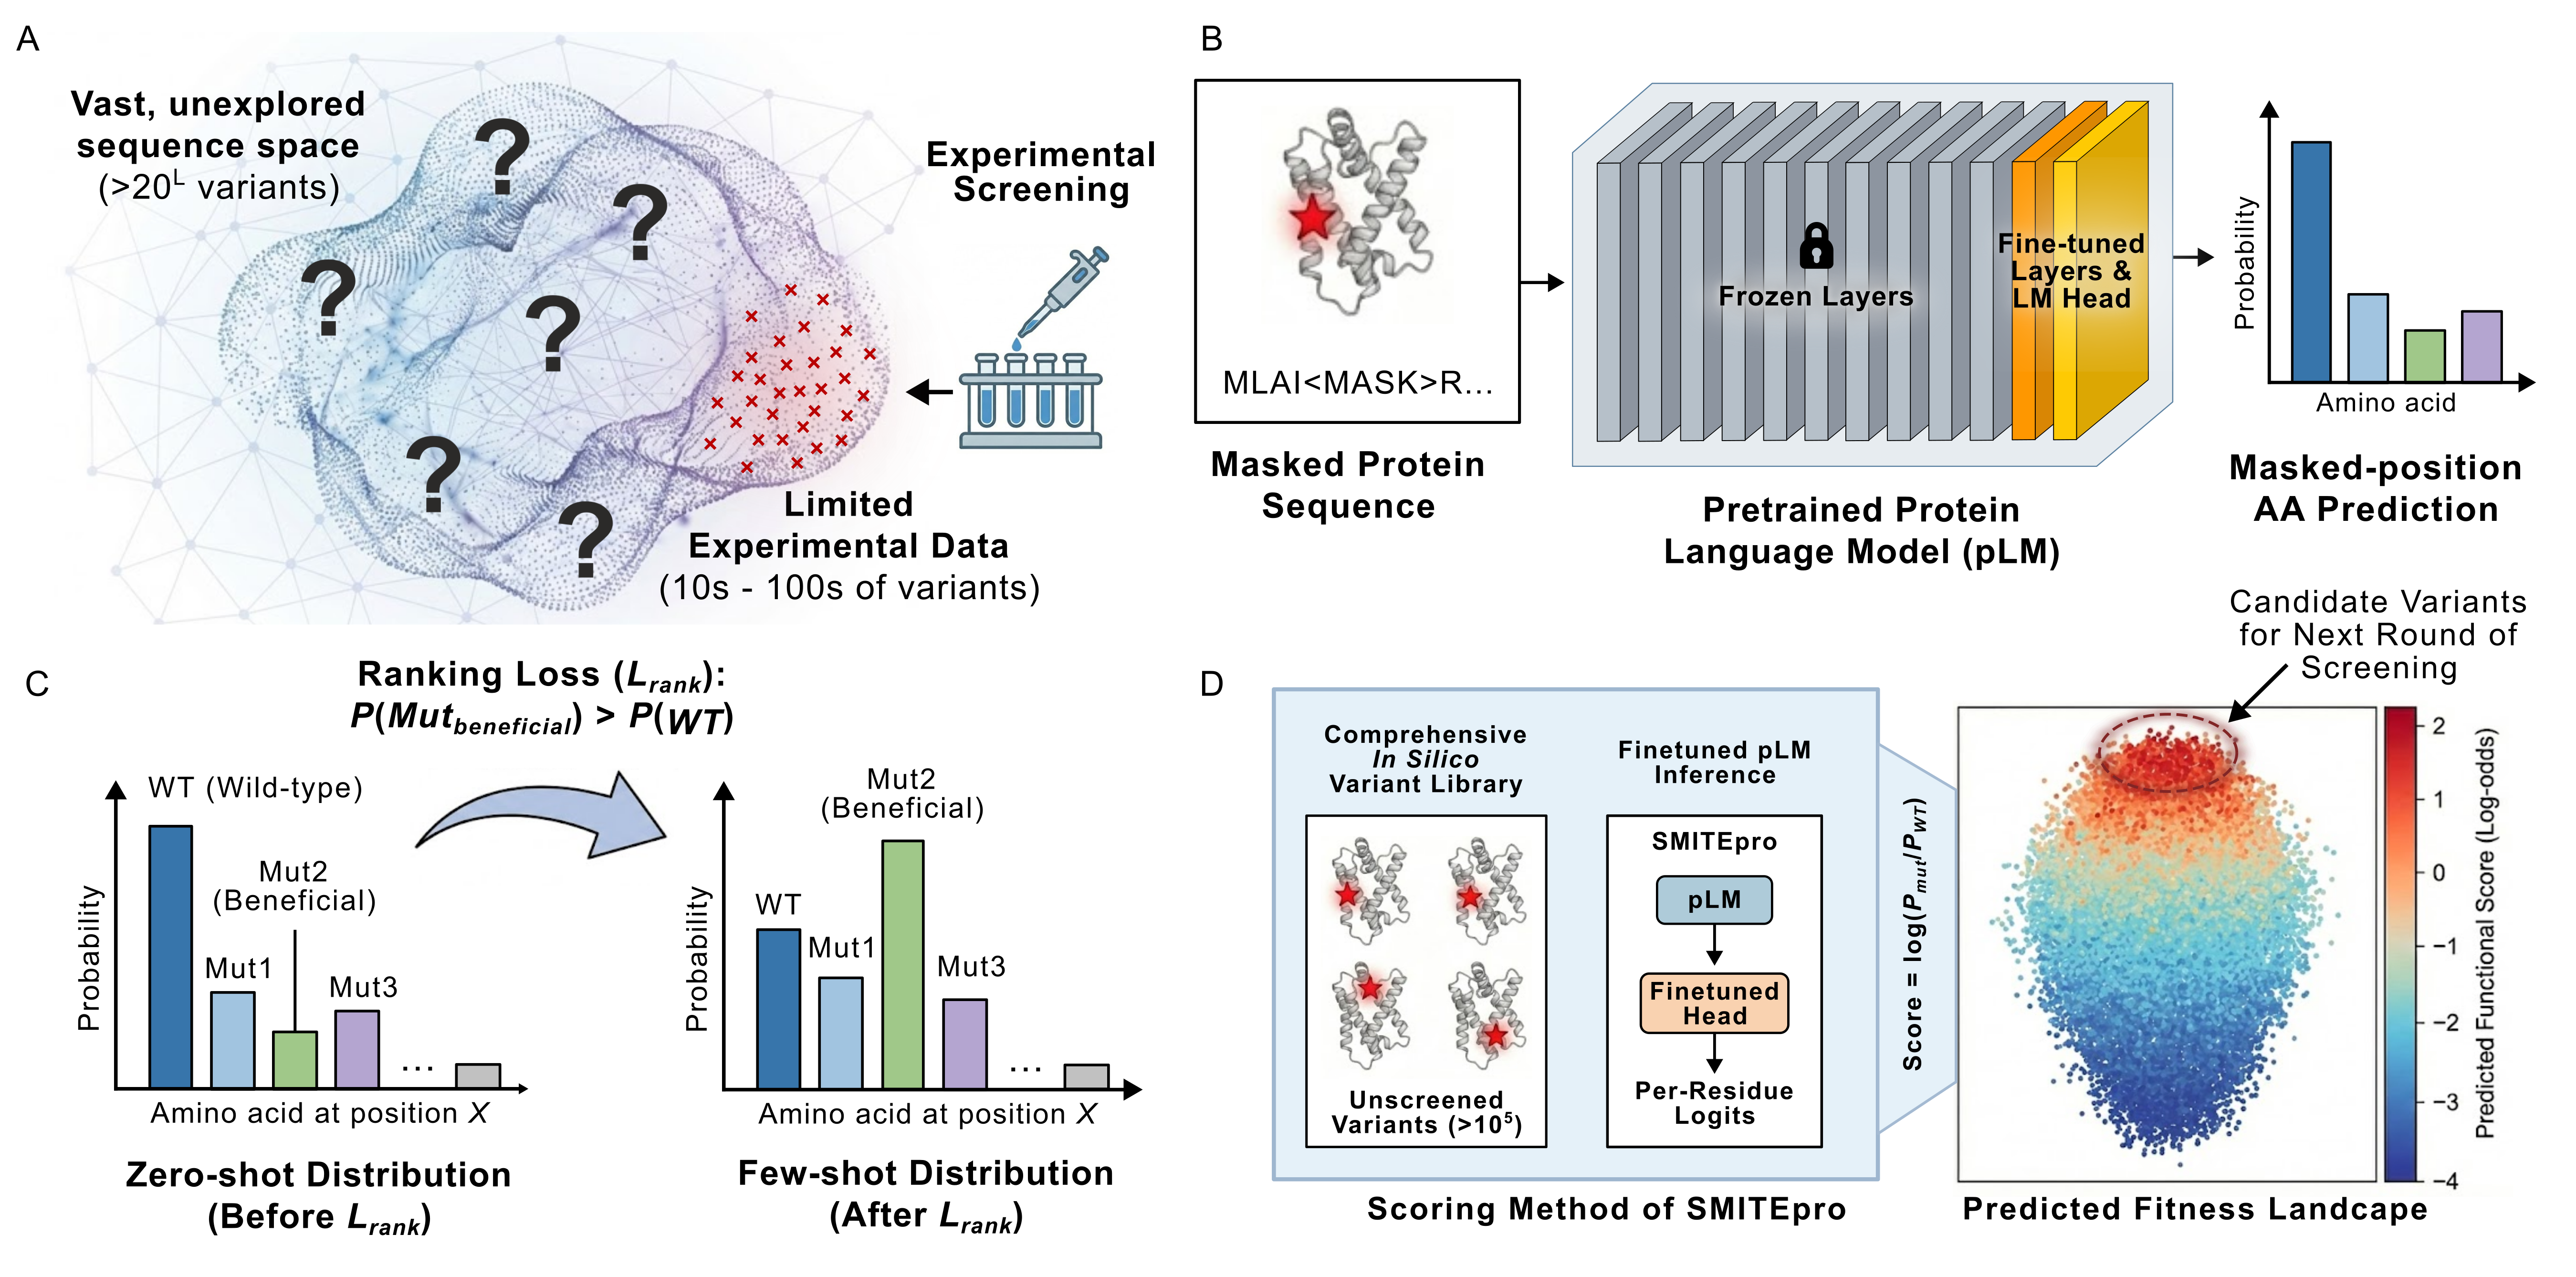
\includegraphics[width=\linewidth]{final_figures/fig1_diagram.png}
    \caption{Overview of the SMITEpro framework for predicting protein fitness landscapes. (A) Limited experimental data covers a small fraction of the vast protein sequence space, making fitness prediction difficult. (B) A pretrained protein language model processes sequences to output per-position amino acid probabilities, providing the initial zero-shot distributions. (C) The ranking loss ($\mathcal{L}_{\text{rank}}$) adjusts these zero-shot probabilities, shifting the few-shot distribution so known beneficial mutations rank higher than the wild-type. (D) The fine-tuned SMITEpro model computes log-odds scores for a comprehensive library of unscreened variants, generating a predicted fitness landscape to identify top candidates for future screening.}
    \label{fig:fig1}
\end{figure}

\subsection{Site-specific scoring extrapolates to unseen sequence positions while global pooling degrades with protein length}

Global regression methods like EVOLVEpro~\cite{jiang2024rapid} rely on dense pretrained ESMC embeddings to predict fitness. However, this method requires compression of the full protein embedding to a single vector, thus diluting site information by taking the average across all positions. Comparing unseen-site ranking performance as a function of protein sequence length directly illustrates this mean-pooling dilution (Figure~\ref{fig:fig2}A). EVOLVEpro is competitive on short domains ($L < 100$) where a single substitution is not completely drowned out by mean-pooling function. In contrast, SMITEpro's advantage at unseen sites scales strongly with protein length ($\rho = 0.45$, $p = 4.1 \times 10^{-11}$ across $n = 197$ assays; Figure~\ref{fig:fig2}A).

We partitioned held-out predictions into \textit{unseen sites} (positions absent from the $K$-variant training set) and \textit{seen sites} (positions with at least one sampled substitution) to reveal how local tuning and global regression diverge when extrapolating to novel regions of the protein (Figure~\ref{fig:fig2}). Understanding this difference is critical for early-stage engineering, where unexplored sequence space heavily outweighs explored regions. In a campaign guided by zero-shot selection, unseen positions dominate the initial search space, comprising 94\%, 88\%, and 75\% of all mutated positions at $K = 16, 32,$ and $64$.

Evaluating 106 benchmark assays with $\ge 100$ mutated positions clarifies how SMITEpro and EVOLVEpro complement each other (complete $K$ scaling in Appendix~\ref{secA2}, Figure~\ref{fig:supp-site-scaling}). At unseen sites, EVOLVEpro struggles with small training sets ($\rho = 0.08 \pm 0.02$ at $K = 16$). Because SMITEpro evaluates the masked distribution directly at the mutated site, it maintains substantially stronger ranking accuracy in these unexplored regions ($\rho = 0.21 \pm 0.01$, Wilcoxon signed-rank $p = 4.9 \times 10^{-10}$). Conversely, at seen sites ($K = 64$), both standalone SMITEpro ($\rho = 0.24 \pm 0.02$) and EVOLVEpro ($\rho = 0.20 \pm 0.01$) interpolate well. Across all held-out sites combined at $K = 64$, standalone SMITEpro ($\rho = 0.24 \pm 0.01$) outperforms EVOLVEpro ($\rho = 0.15 \pm 0.02$). Ultimately, their equal-weight ensemble captures the best of both approaches, achieving the highest overall correlation ($\rho = 0.25 \pm 0.02$; Figure~\ref{fig:fig2}B).

Finally, expanding the training size from $K = 16$ to $128$ introduces a depletion effect. Because the initial training variants are selected from top zero-shot predictions, increasing $K$ systematically shifts the most beneficial sequence positions out of the unseen pool and into the seen partition. Even as the remaining unseen pool becomes depleted of high-fitness variants, SMITEpro accurately recognizes that the seen-site variants are superior. It places them high in the global predicted rankings (between the 68th and 84th percentiles of all predicted fitness scores), whereas EVOLVEpro scores them near the middle of the pack (52nd to 53rd percentile). This accurate global sorting drives the steady improvement of the ensemble across the complete library as data scales from $K = 16$ to $K = 128$ ($\rho = 0.19 \rightarrow 0.20 \rightarrow 0.25 \rightarrow 0.31$; Figure~\ref{fig:supp-site-scaling}C).

\begin{figure}[htbp]
    \centering
    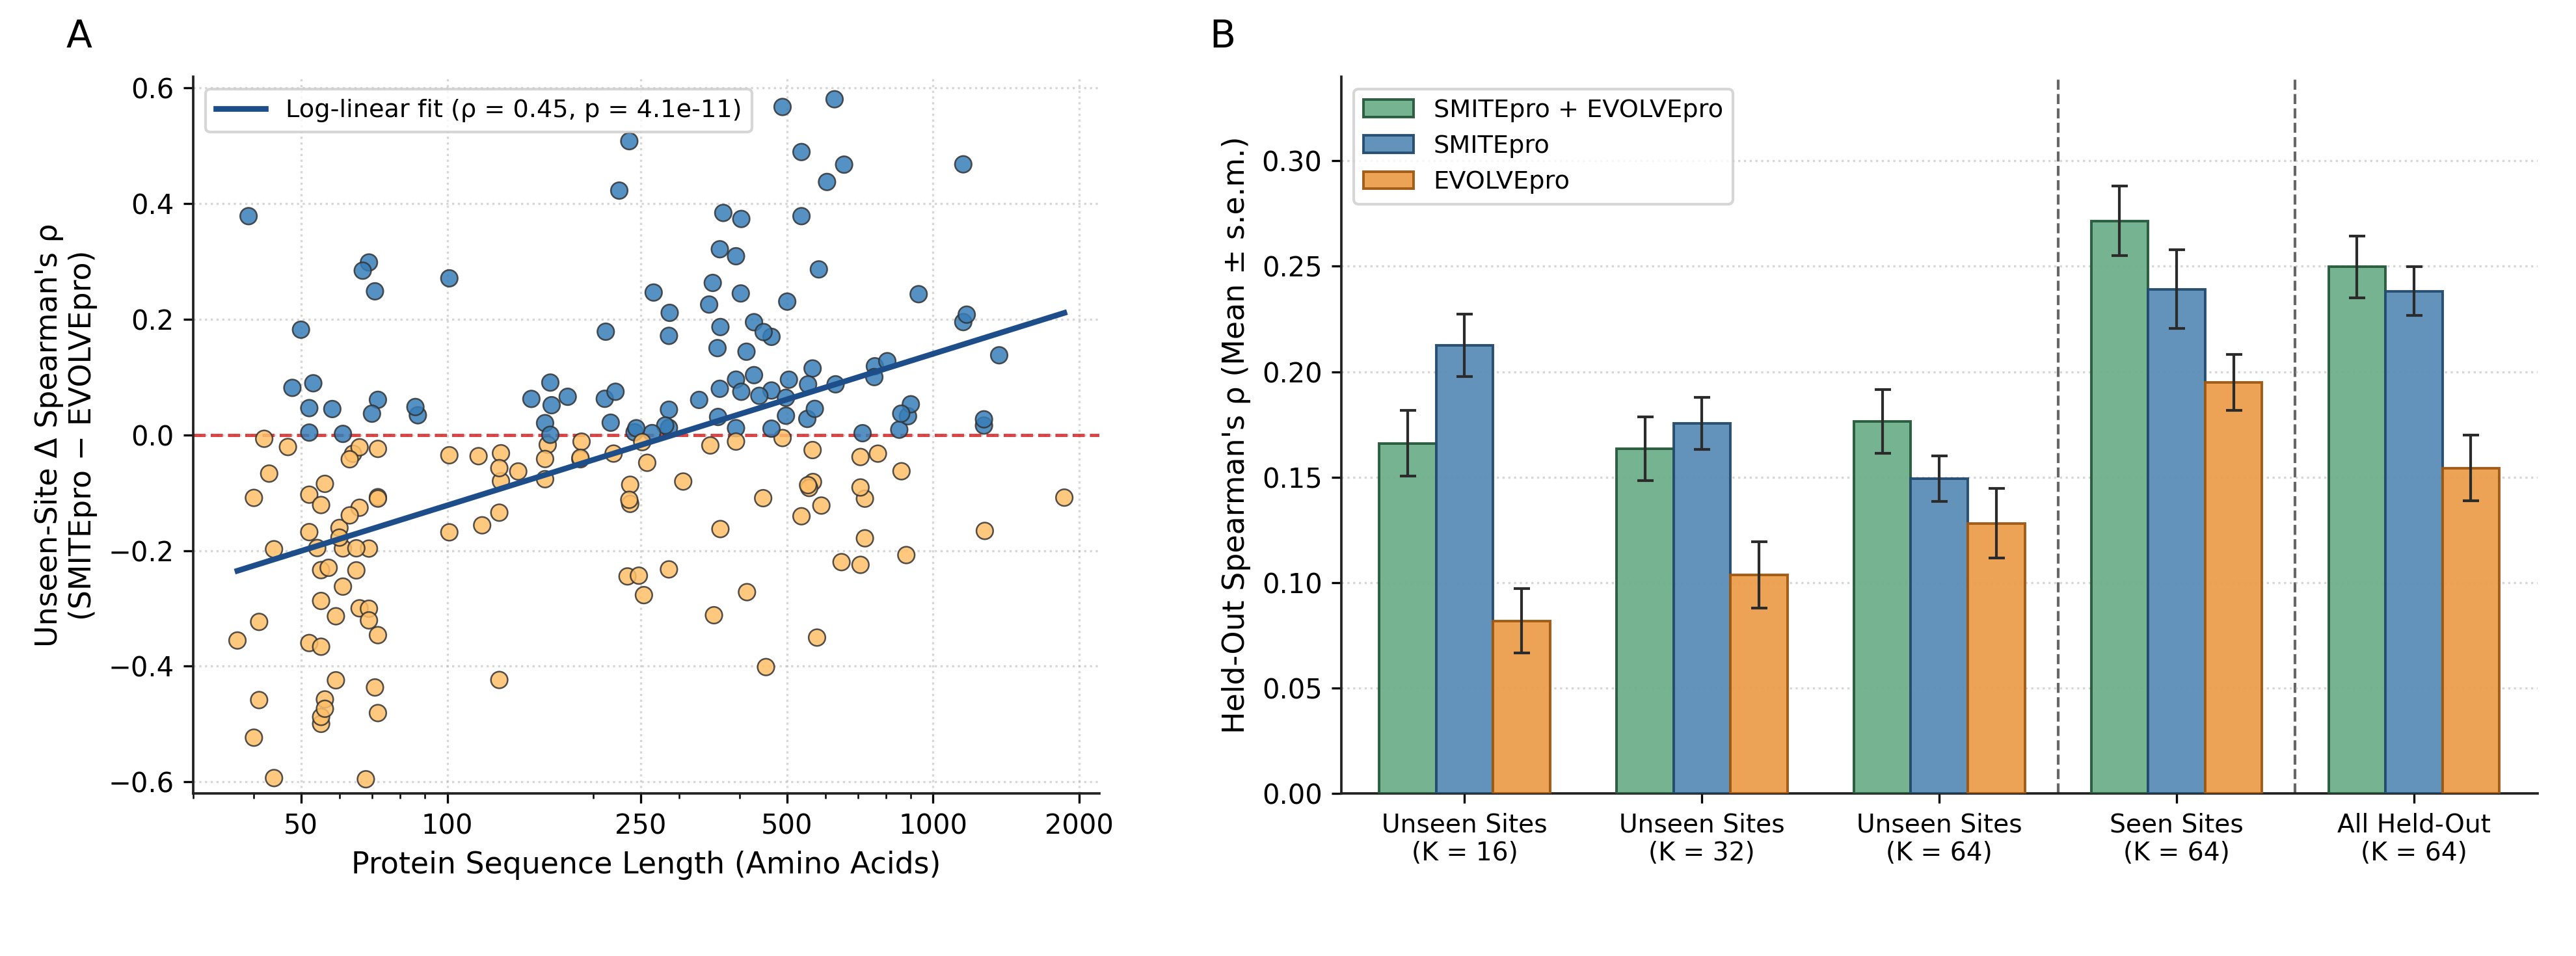
\includegraphics[width=\linewidth]{final_figures/fig2_spearman.png}
    \caption{Site-level evaluation at unseen versus seen sequence positions across ProteinGym assays. (A) Difference in unseen-site Spearman's rank correlation ($\Delta\text{Spearman's }\rho = \text{SMITEpro} - \text{EVOLVEpro}$ at $K = 32$) plotted against protein sequence length $L$ (log scale; $n = 197$ assays with unseen sites). The solid line shows the log-linear trend ($\rho = 0.45$, $p = 4.1 \times 10^{-11}$), and the red dashed line marks equal performance. (B) Mean held-out Spearman's rank correlation ($\rho \pm \text{s.e.m.}$) across the 106 benchmark assays ($\ge 100$ mutated positions) partitioned into unseen sites (positions absent from the training set at training sizes $K = 16, 32,$ and $64$), seen sites (positions mutated in the training set at $K = 64$), and all held-out sites combined ($K = 64$) for the equal-weight SMITEpro + EVOLVEpro ensemble, SMITEpro, and EVOLVEpro.}
    \label{fig:fig2}
\end{figure}

\subsection{SMITEpro and its ensemble improve recovery of highly functional variants}

Practical directed evolution campaigns often face bottlenecks in functional assays, driving a shift toward low-$N$ pick-and-validate loops where only a small number of top-ranked candidates are screened per round~\cite{chu2024accurate, yang2025active}. Therefore, we benchmarked top-$N$ variant discovery across training set sizes of $K \in \{16, 32, 64, 128\}$ (at our prospective screening budget of $N = 20$; Figure~\ref{fig:fig3}A,C) and screening budgets of $N \in \{10, 20, 30, 40\}$ variants (Figure~\ref{fig:fig3}B,D). We compared SMITEpro against EVOLVEpro~\cite{jiang2024rapid}, a sequence-kernel Gaussian process (Kermut)~\cite{groth2024kermut}, an alignment-based position-specific score matrix (PSSM)~\cite{gribskov1987profile}, zero-shot ESMC~\cite{esm2024cambrian}, and a random baseline. We focused on the 106 ProteinGym single-substitution assays containing substitutions at at least 100 distinct positions with complete results across all methods and training sizes. This criterion ensured sufficient mutation-site coverage. We evaluated both the top 1\% enrichment factor over the held-out pool (Figure~\ref{fig:fig3}A,B) and the mean selected normalized fitness (Figure~\ref{fig:fig3}C,D).

With an experimental screening budget of 20 mutations, standalone SMITEpro consistently outperformed all individual baselines in top 1\% enrichment across every training set size. SMITEpro achieved a $3.80 \pm 0.56$-fold enrichment at $K = 16$ (vs. $2.26 \pm 0.34$-fold for EVOLVEpro) and rose to $4.60 \pm 0.49$-fold at $K = 128$ (vs. $3.24 \pm 0.41$-fold for EVOLVEpro; Figure~\ref{fig:fig3}A). It also maintained high mean selected fitness even at the smallest training set size, reaching $0.38 \pm 0.03$ at $K = 16$ compared to $0.28 \pm 0.03$ for EVOLVEpro (Figure~\ref{fig:fig3}C).

Combining SMITEpro with EVOLVEpro in an equal-weight ensemble achieved the highest performance across nearly every training size and selection budget. The ensemble yielded a mean rank of 1.03 across the 32 $(K, N, \text{metric})$ settings, followed by standalone SMITEpro (2.12), EVOLVEpro and Gaussian process regression (tied at 4.12), MSA PSSM (4.31), zero-shot ESMC (5.28), and random selection (7.00; Figure~\ref{fig:fig3}). At $N = 20$, the ensemble increased top 1\% enrichment from $4.51 \pm 0.72$-fold at $K = 16$ to $5.53 \pm 0.63$-fold at $K = 128$ (Figure~\ref{fig:fig3}A). Mean selected fitness likewise improved from $0.46 \pm 0.03$ to $0.51 \pm 0.03$ (Figure~\ref{fig:fig3}C). This clear lead across all screening budgets ($N = 10$ to $N = 40$; Figure~\ref{fig:fig3}B,D) motivated its prospective deployment for enzyme engineering.

\begin{figure}[htbp]
    \centering
    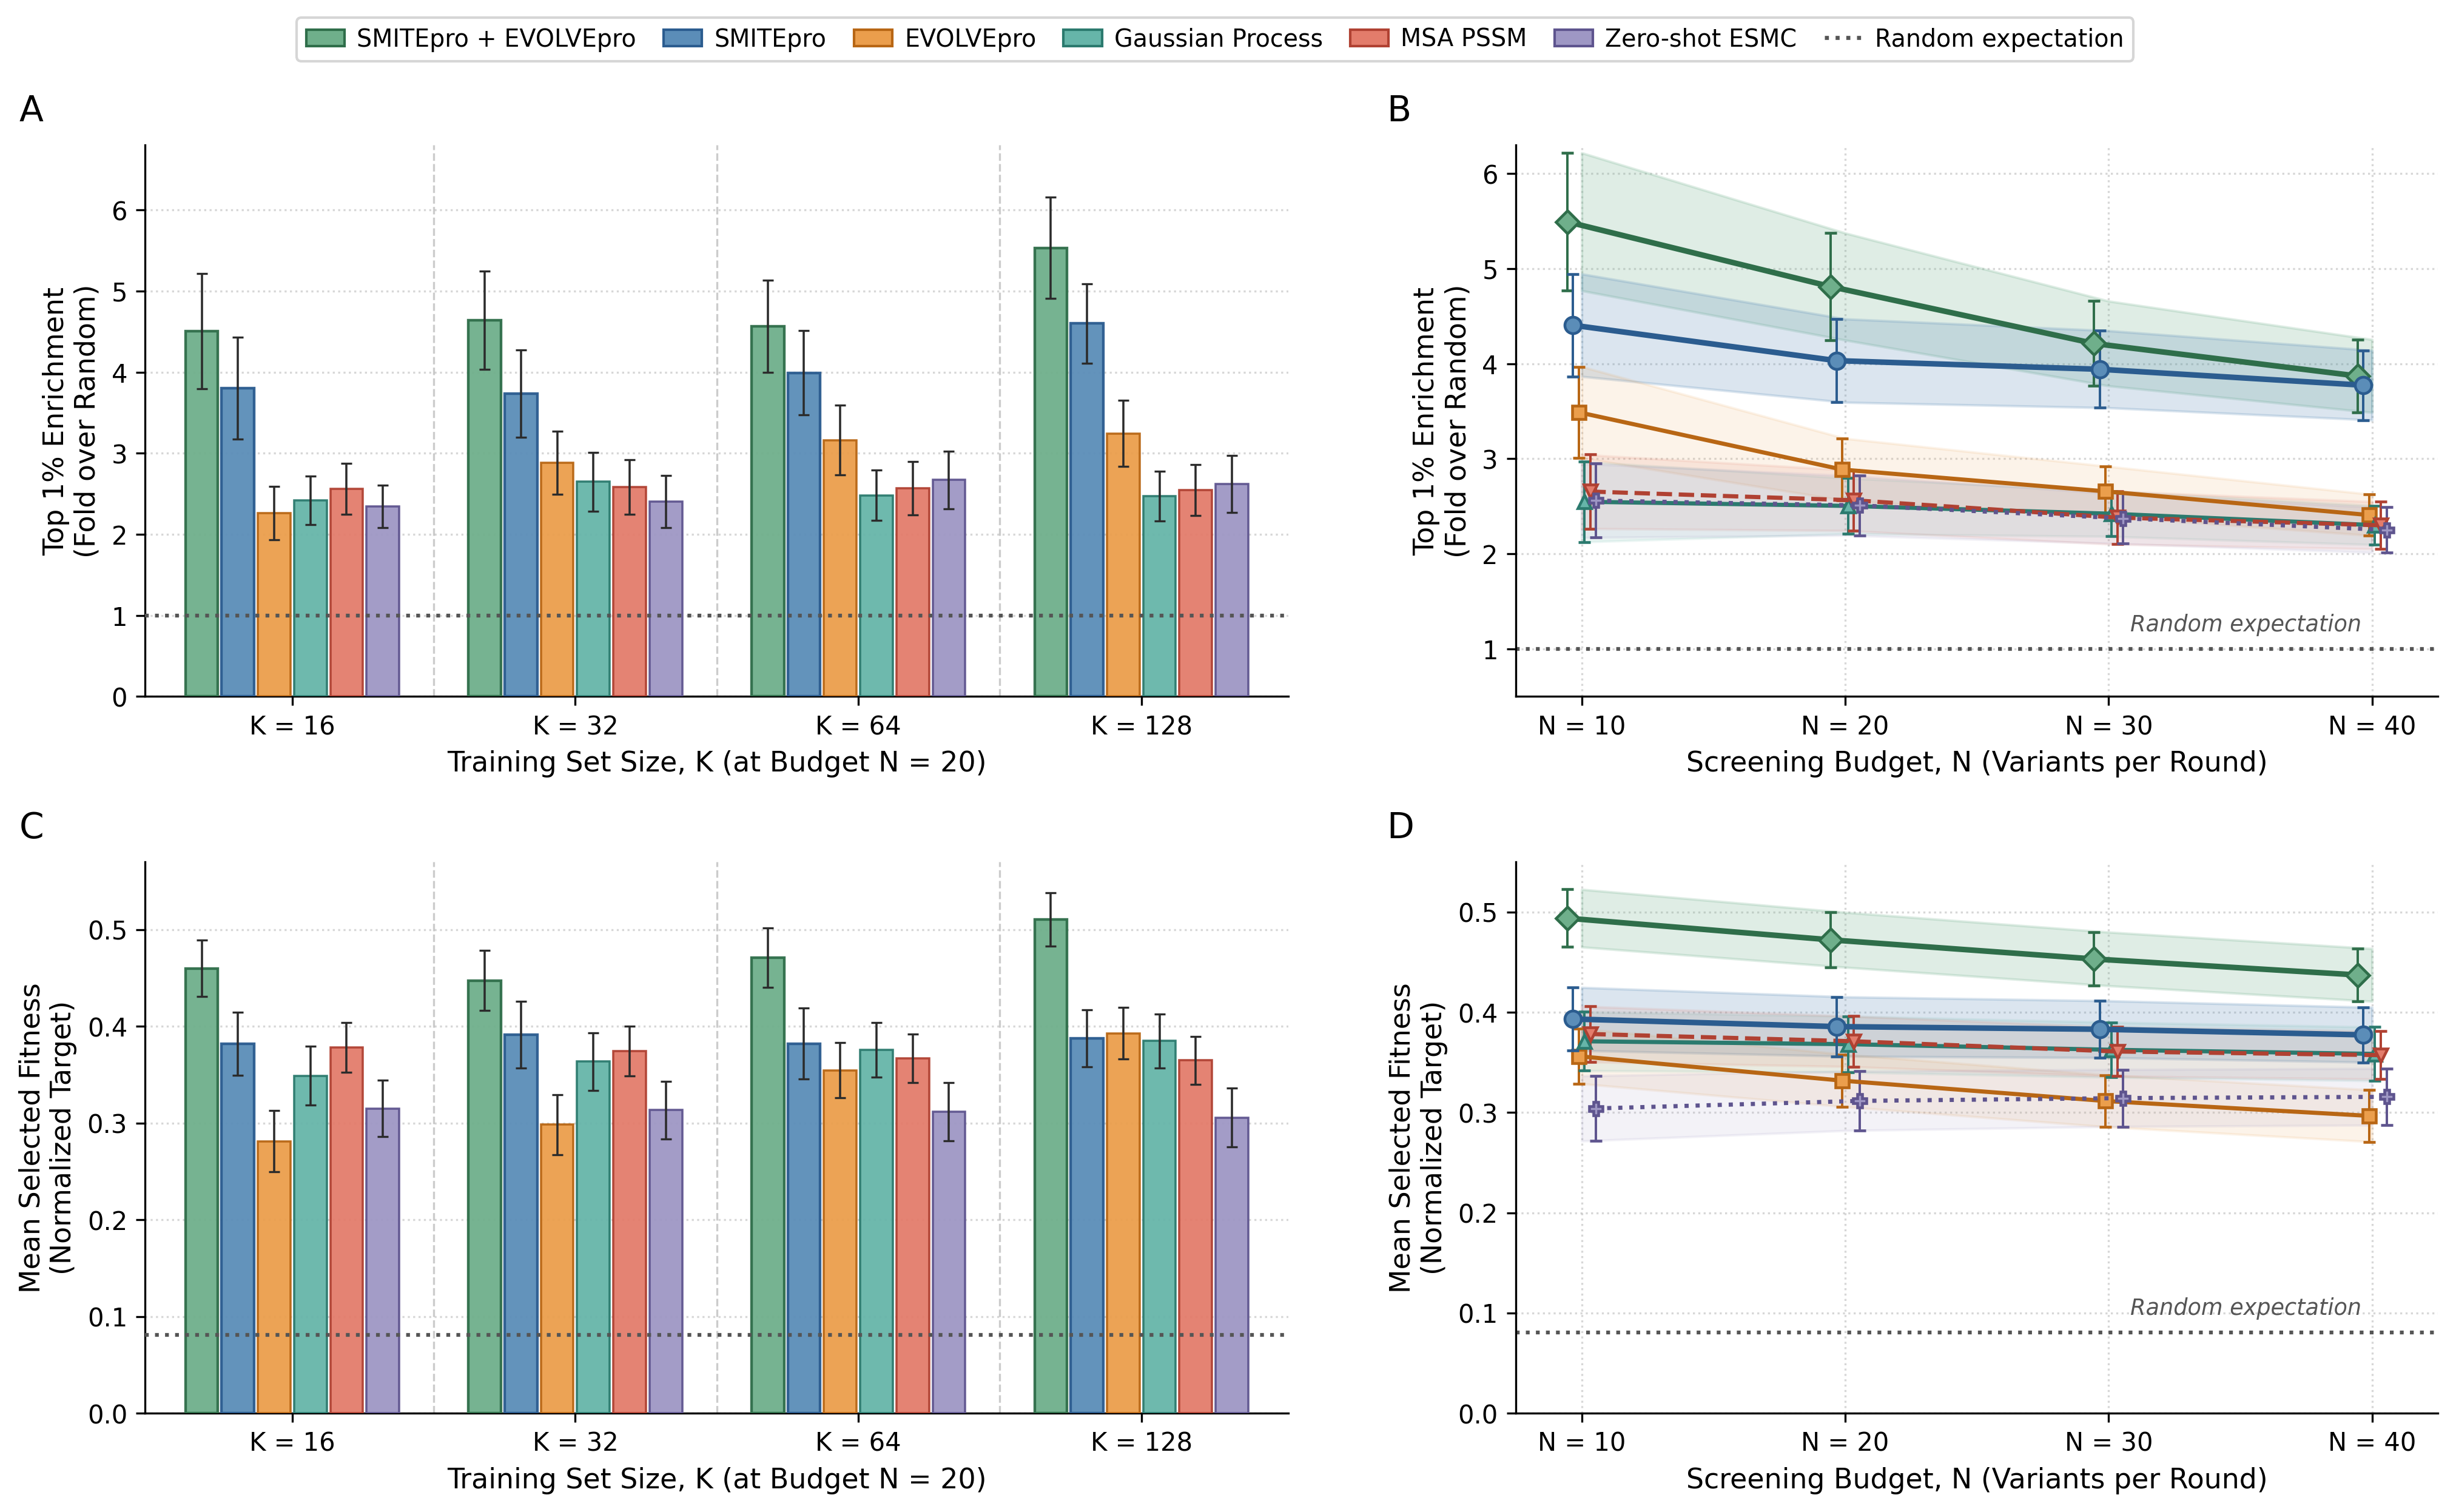
\includegraphics[width=\linewidth]{final_figures/fig3_enrichment.png}
    \caption{Top-$N$ variant discovery across training set sizes and screening budgets on 106 ProteinGym assays ($\ge 100$ mutated positions). (A) Top 1\% enrichment factor ($\pm\text{s.e.m.}$ across $n = 106$ assays) at the $N = 20$ screening budget across training set sizes $K \in \{16, 32, 64, 128\}$. (B) Top 1\% enrichment factor across screening budgets $N \in \{10, 20, 30, 40\}$ averaged across training sizes $K$ within each assay; shaded bands indicate $\pm\text{s.e.m.}$ across assays. (C) Mean selected normalized fitness ($\pm\text{s.e.m.}$) at $N = 20$ across training set sizes $K \in \{16, 32, 64, 128\}$. (D) Mean selected normalized fitness across screening budgets $N \in \{10, 20, 30, 40\}$ ($\pm\text{s.e.m.}$). Horizontal dotted lines in all panels mark the $K$- and $N$-invariant random expectation ($1.0\times$ enrichment in A,B and mean pool fitness $0.081$ in C,D).}
    \label{fig:fig3}
\end{figure}

\subsection{Engineering HpaBC for L-DOPA production}

We applied the equal-weight SMITEpro-EVOLVEpro ensemble to engineer the \textit{Escherichia coli} 4-hydroxyphenylacetate 3-monooxygenase (HpaBC) system for enhanced L-DOPA biosynthesis~\cite{wei2016genome}. To evaluate the modeling approach and bypass the extended timelines of iterative screening, the hybrid model was trained on two HpaB mutational datasets previously evaluated in the same fluorescent system used in this study~\cite{gilmour2025directed, gutierrez2026monooxygenase}. Our experimental design strictly excluded any mutations that had already been measured and included in the training data. This forced the ensemble to predict entirely novel, uncharacterized substitutions for every background. 

\begin{figure}[htbp]
    \centering
    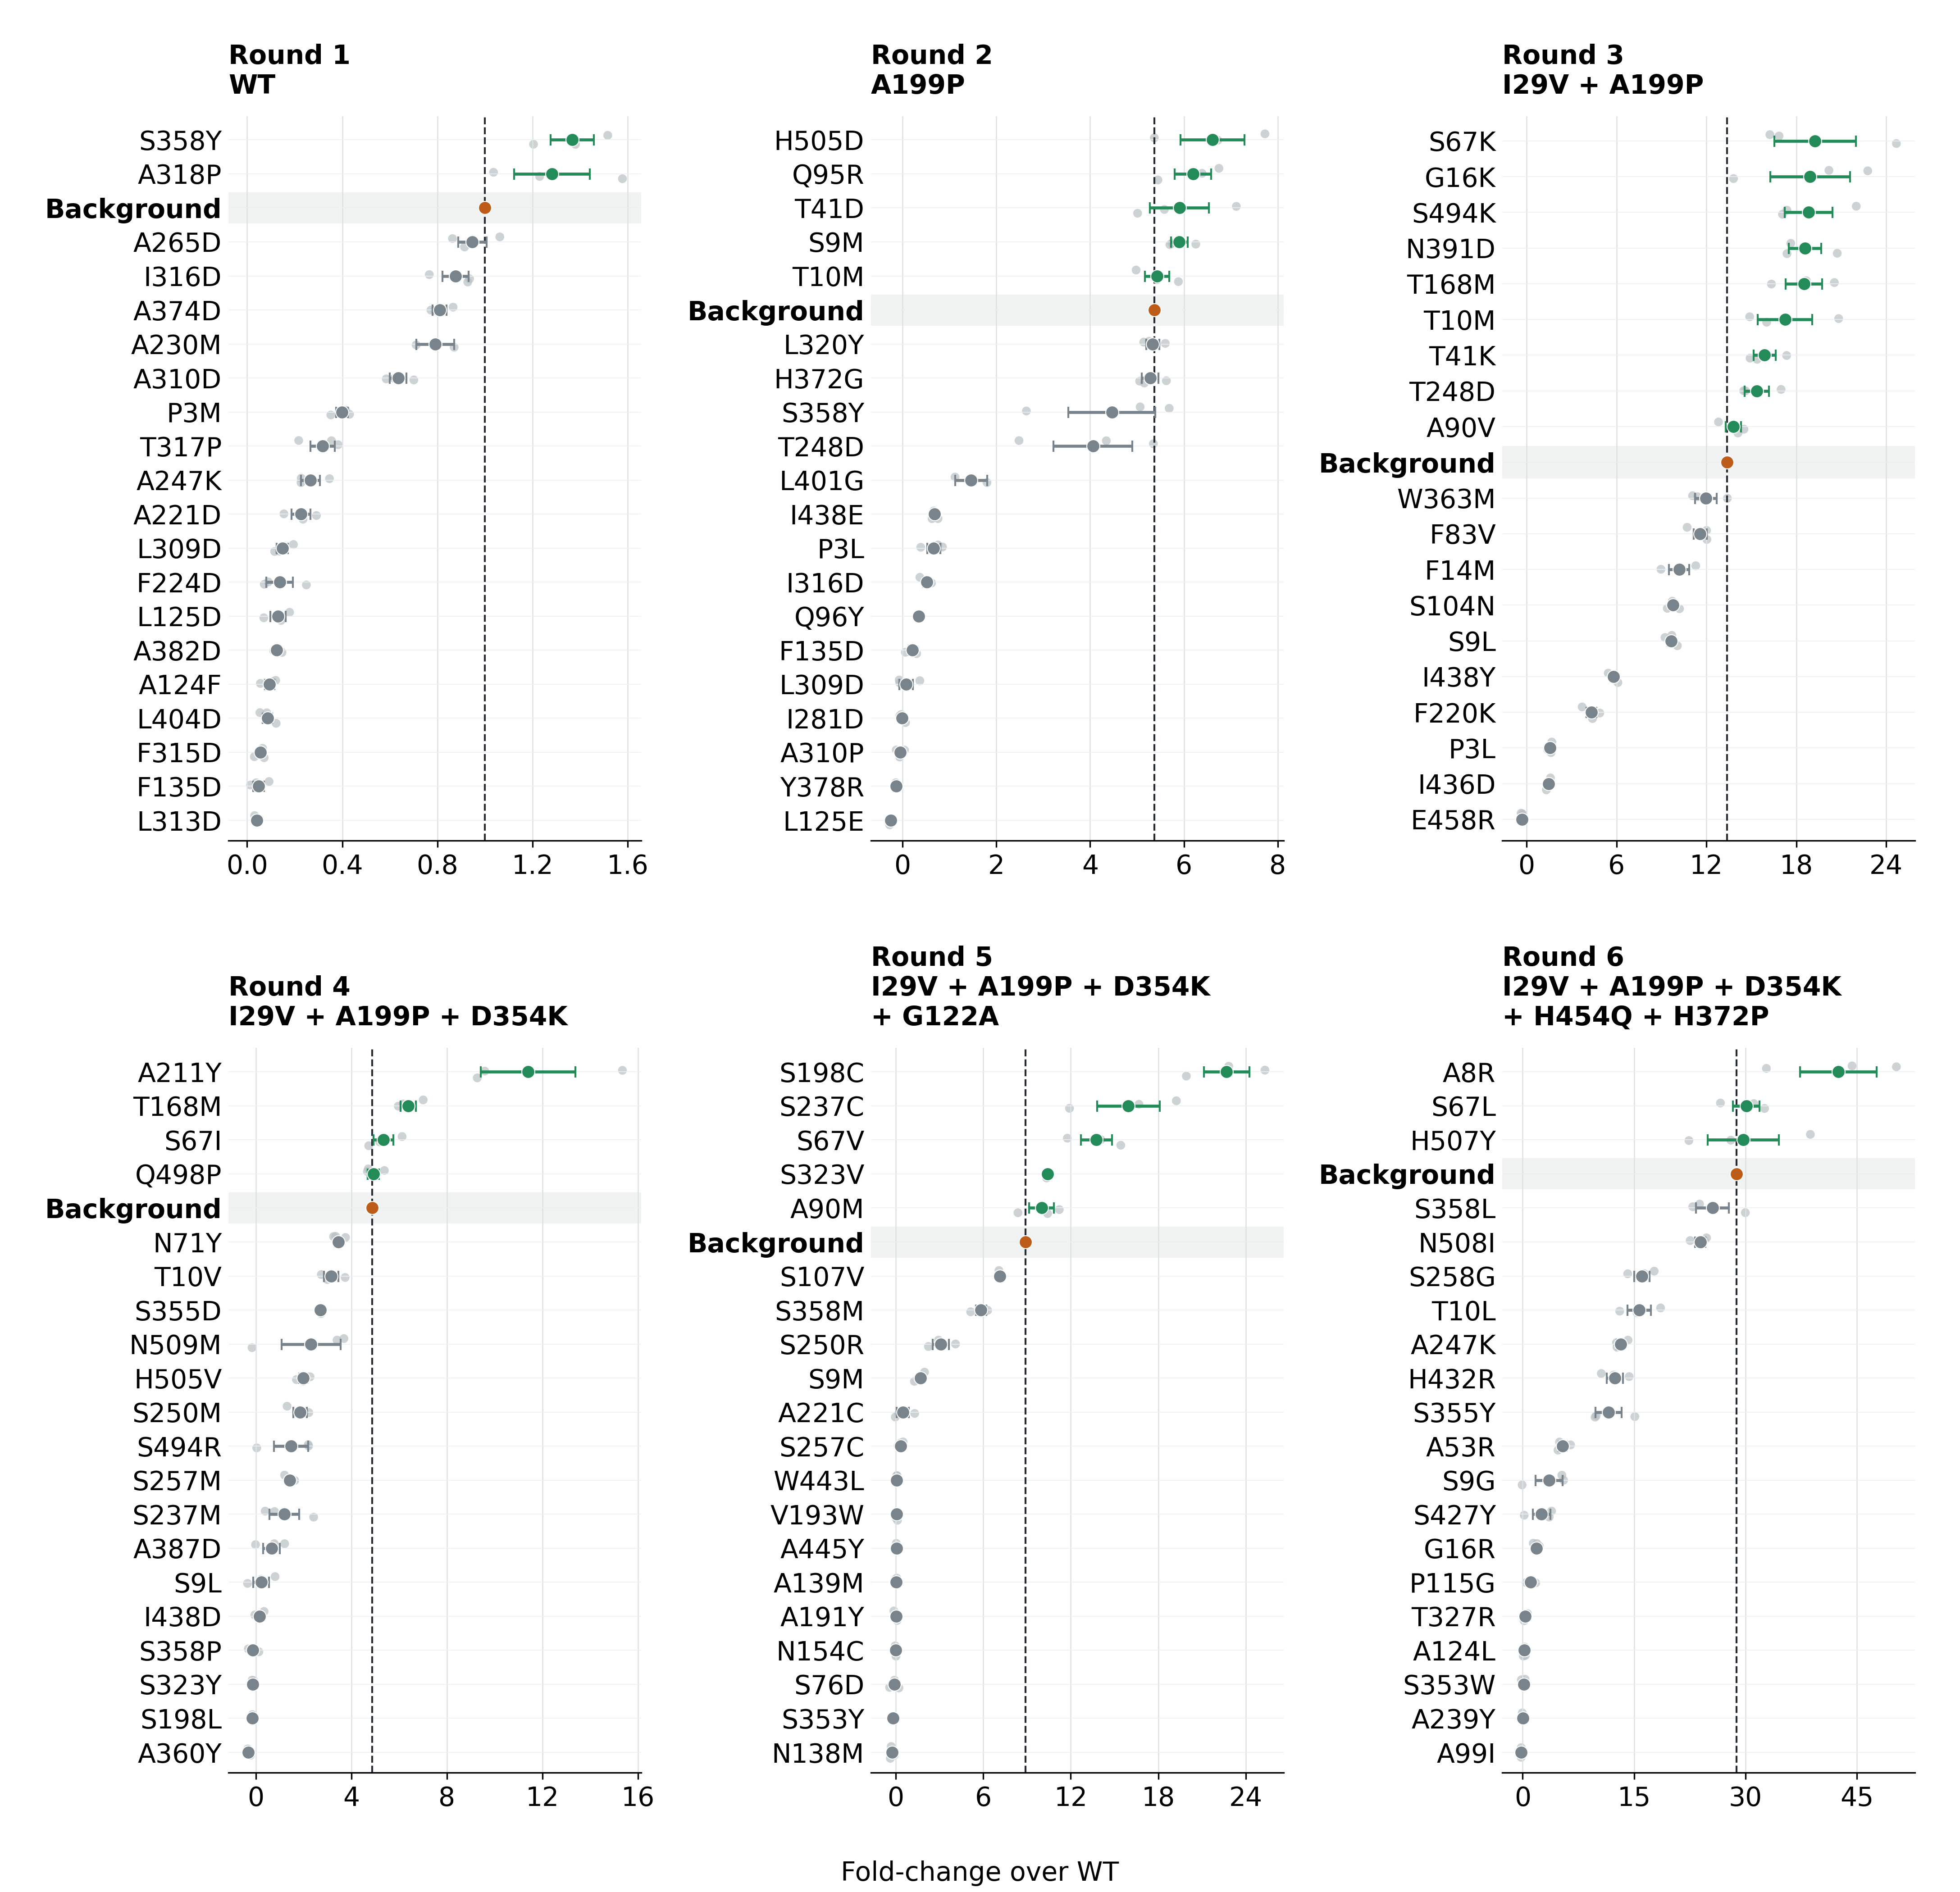
\includegraphics[width=0.99\linewidth]{final_figures/fig4_hpab_experiment.png}
    \caption{Experimental result of mutations to HpaBC for L-DOPA production across six parental backgrounds. Each panel displays the 20 top-ranked single-amino-acid substitutions (19 in Round 3) selected by the SMITEpro--EVOLVEpro ensemble on the indicated parental background, plotted on independently scaled linear WT-relative axes. Gray dots show individual plate-matched biological replicate measurements; colored circles and horizontal bars show the arithmetic mean $\pm$ s.e.m.\ ($n=3$ single-plate replicates for 112 of 119 candidates). Orange circles and vertical dashed lines mark each round's parental background control at its calibrated WT-relative activity; green circles denote variants whose mean activity exceeded the matched parental background, and dark gray circles denote variants at or below the parental background.}
    \label{fig:fig4}
\end{figure}

We then used the trained ensemble to score and rank all untested single-amino-acid substitutions across six progressively mutated HpaB backgrounds. The target backgrounds included: wild-type ($1.00\times$ WT), A199P ($5.37\times$ WT), I29V+A199P ($13.38\times$ WT), I29V+A199P+D354K ($4.88\times$ WT), I29V+A199P+D354K+G122A ($8.91\times$ WT), and I29V+A199P+D354K+H454Q+H372P ($28.78\times$ WT). Of the 120 planned variants, 119 were successfully cloned and assayed concurrently in plate-matched biological triplicates using an L-DOPA-responsive GFP biosensor circuit (I29V+A199P+A53R was not recovered; Figure~\ref{fig:fig4}).

Across all six backgrounds, 28 of the 119 tested candidates (23.5\%) exceeded the mean L-DOPA fluorescence of their matched parental background, and 67 (56.3\%) exceeded wild-type HpaBC activity (Figure~\ref{fig:fig4}). On the wild-type background (Background 1), two variants exceeded WT, led by S358Y ($1.37\times$ WT) and A318P ($1.28\times$ WT). Hit rates were substantially higher on the previously evolved backgrounds. On the A199P background (Background 2), five variants exceeded the parental enzyme (led by H505D at $1.23\times$ background, or $6.61\times$ WT). Background 3 (I29V+A199P) yielded our highest hit rate, with 9 of 19 candidates (47.4\%) exceeding the parental baseline (led by S67K at $19.25\times$ WT, G16K at $18.92\times$ WT, and S494K at $18.82\times$ WT).

The ensemble continued to identify improved variants even as the fitness landscape grew more constrained on the heavily mutated backgrounds. On the I29V+A199P+D354K background (Background 4), four candidates improved over the parental baseline, with A211Y achieving a $2.34\times$ improvement ($11.40\times$ WT). On the quadruple-mutant background (Background 5), five candidates exceeded the parental baseline, led by S198C ($22.68\times$ WT), S237C ($15.94\times$ WT), and S67V ($13.75\times$ WT). Finally, on the highly active quintuple-mutant background (Background 6, $28.78\times$ WT), three candidates surpassed the parental control. The top sextuple variant, adding A8R, reached a 42.49-fold improvement in L-DOPA biosensor signal over wild-type HpaBC (alongside S67L at $30.09\times$ WT and H507Y at $29.71\times$ WT).

\subsection{Post-hoc stability predictions help interpret the experimental outcomes}

Although the ensemble identified beneficial substitutions on every background, the fraction of candidates falling below the parental baseline increased as mutations stacked (15 of 20 on Background 5; 17 of 20 on Background 6). Sequence-only models trained on functional readouts do not explicitly track cumulative thermodynamic stability. Therefore, we hypothesized that the highly evolved HpaB backgrounds had exhausted their stability margins, leaving subsequent substitutions vulnerable to unfolding. To test this, we used the structure-informed stability predictor StabilityArc\cite{feller2026stabilityarc} to retrospectively score all 119 tested substitutions on their specific HpaB backgrounds (Figure~\ref{fig:hpab-stability}).

The post-hoc stability analysis supports this dynamic. Across the entire campaign, 52 of the 91 variants measuring below their matched background were predicted to be destabilizing (StabilityArc score $< 0$). In contrast, only 4 of the 28 improved variants were predicted to be destabilizing. This separation was striking on the five previously evolved backgrounds (Backgrounds 2 through 6). Of the 41 predicted destabilizing substitutions tested on these evolved backgrounds, 38 (92.7\%) failed to improve over their parental control. Two of the three exceptions (T41K on Background 3 at $-0.004$ and S237C on Background 5 at $-0.003$) had virtually neutral stability scores.

These results suggest that fold destabilization may contribute to many of the experimental failures. Pairing the SMITEpro and EVOLVEpro ensemble with an explicit stability filter could help mitigate this risk and further improve hit rates in deep mutational trajectories.

\begin{figure}[htbp]
    \centering
    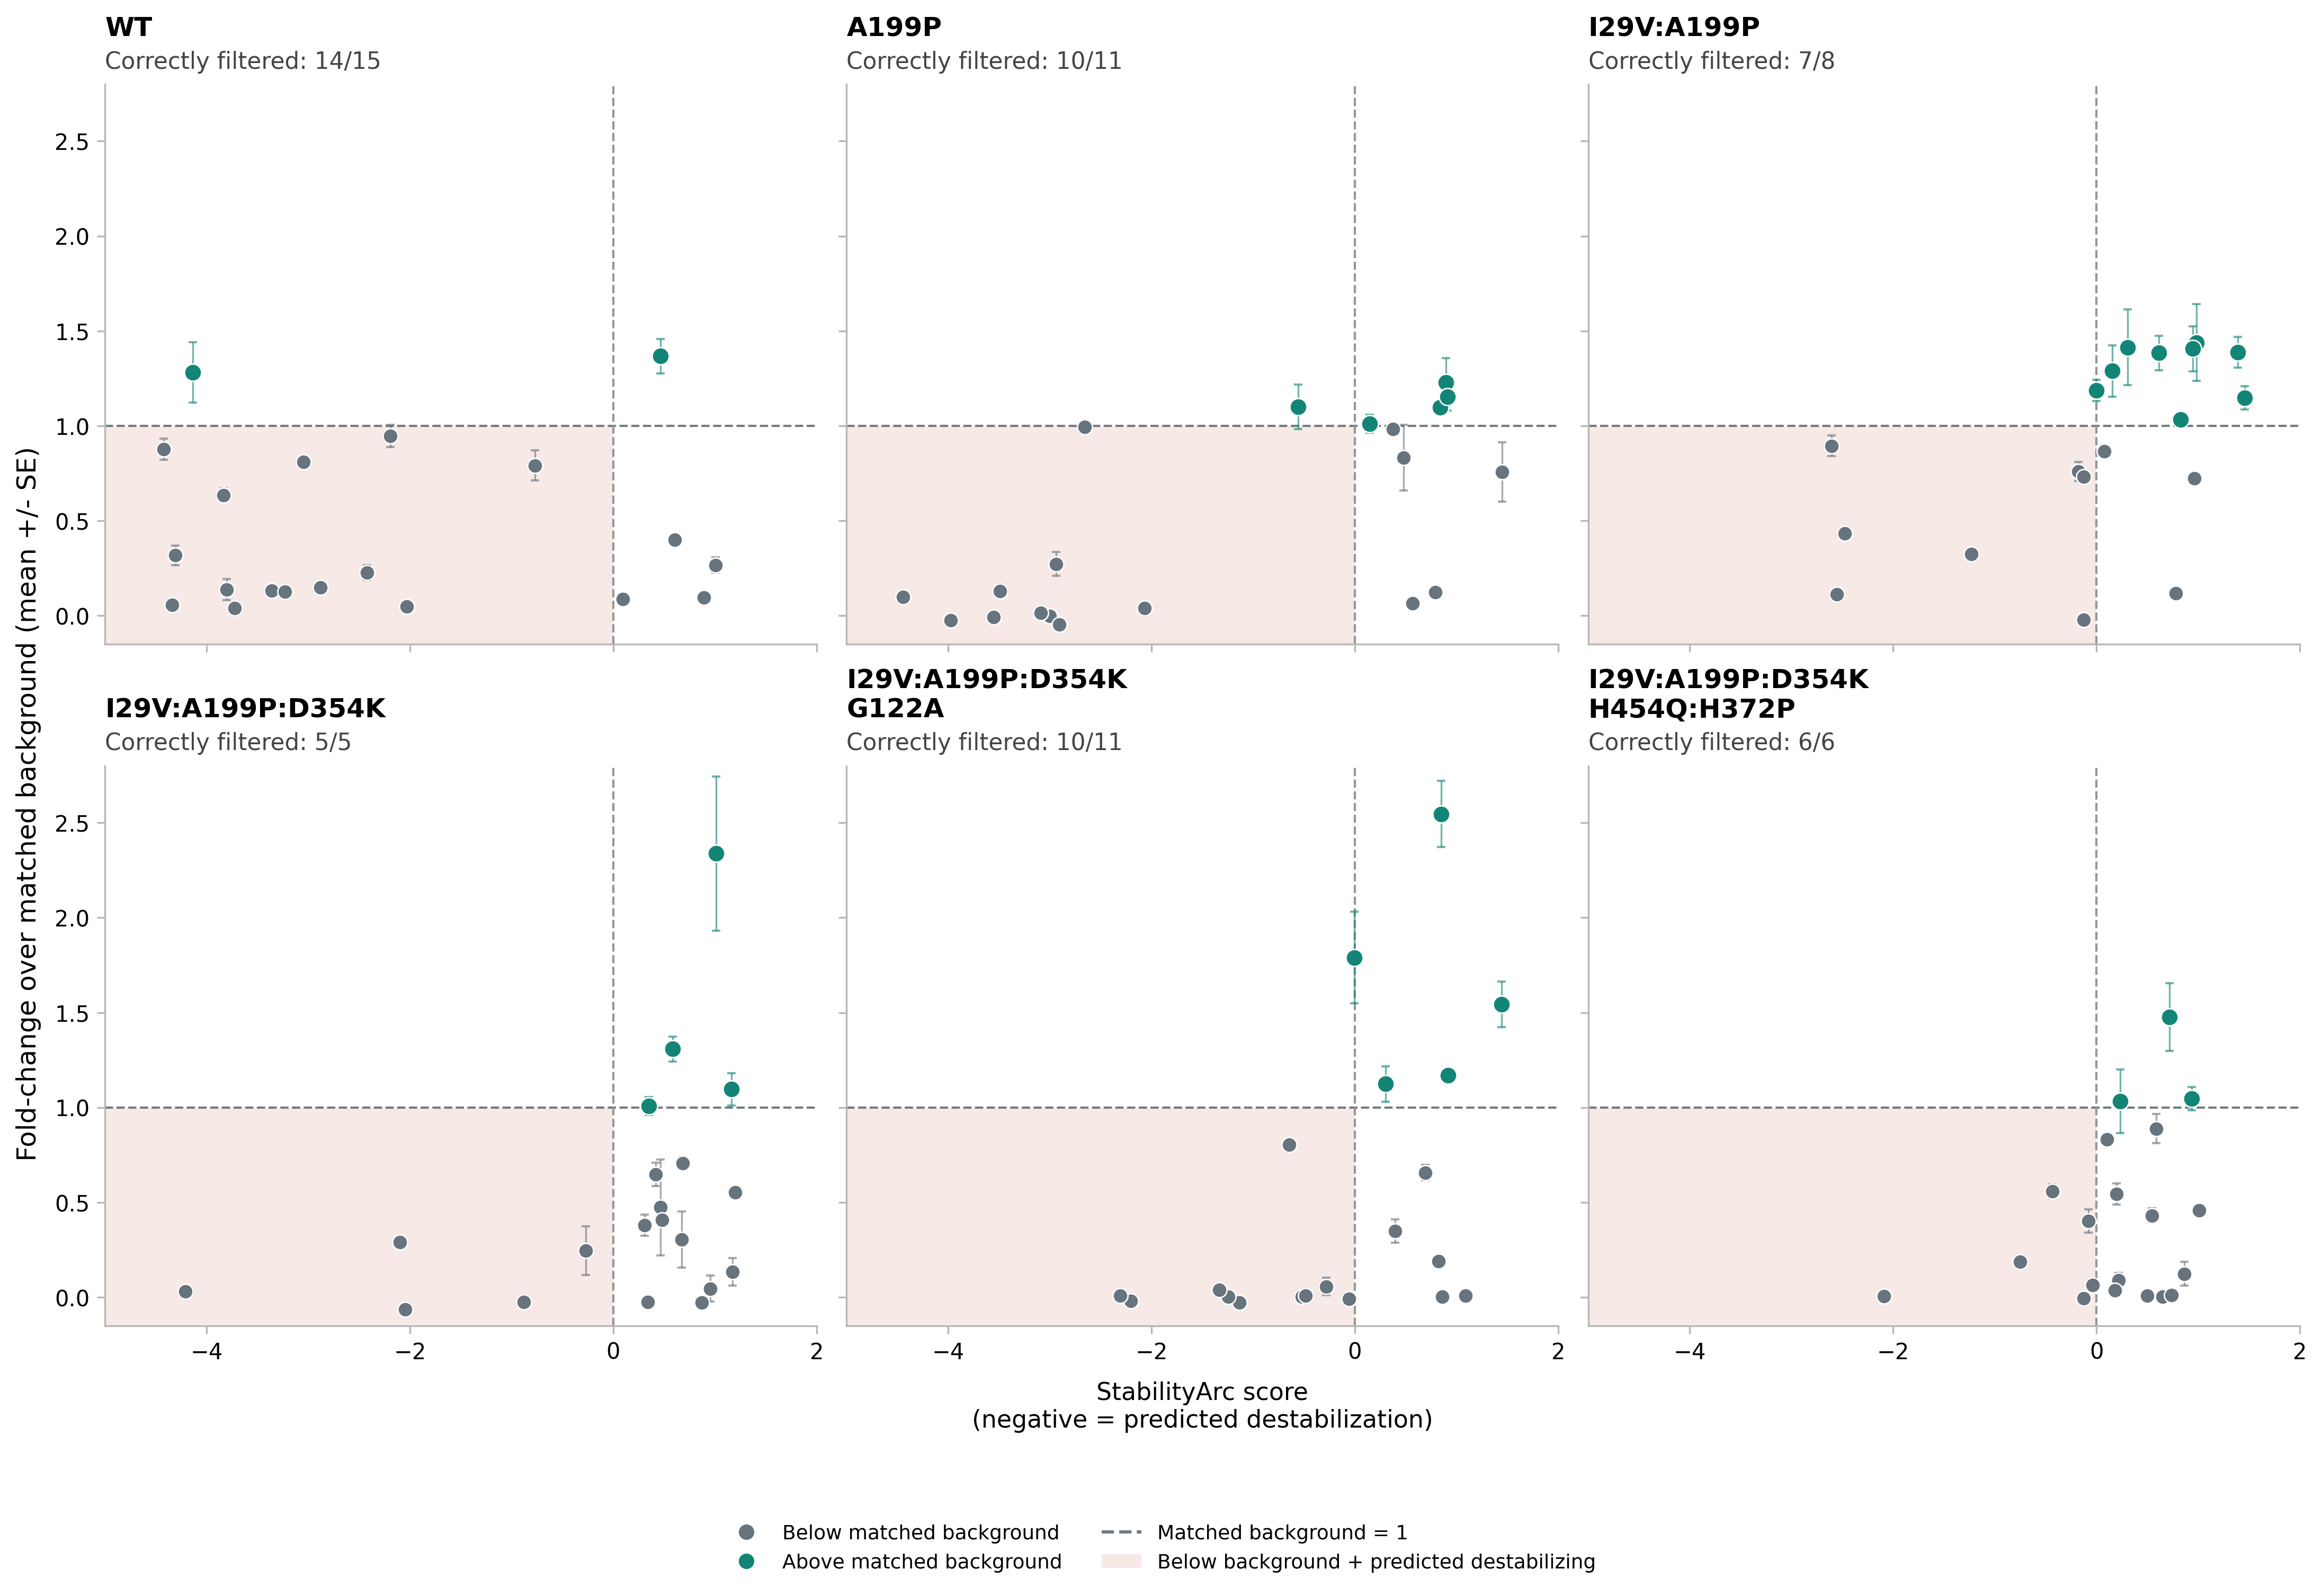
\includegraphics[width=\linewidth]{final_figures/fig5_hpab_stability.png}
    \caption{Post-hoc comparison of predicted thermodynamic stability and experimental outcome across six HpaB backgrounds. Each point represents one tested single substitution ($n=119$ total across panels A--F), scored by StabilityArc on its corresponding experimental background. Vertical error bars indicate mean $\pm$ s.e.m.\ from plate-matched biological replicates relative to the parental background. Gray circles indicate variants measured below the matched background; teal circles indicate variants exceeding the matched background. Horizontal dashed lines mark the matched parental background ($\text{fold-change} = 1.0$), and vertical dashed lines mark a neutral StabilityArc score ($0.0$, where negative values indicate predicted destabilization). The shaded pink quadrant highlights variants that were both predicted destabilizing and measured below their parental background. Each panel reports the number of tested variants and Spearman's rank correlation ($\rho$).}
    \label{fig:hpab-stability}
\end{figure}

\section{Discussion}

Protein engineering with limited data forces a trade-off between the broad generalization of zero-shot models and the task-specific precision of supervised methods. SMITEpro bridges this gap by adapting a pretrained model's residue-level predictions directly to experimental measurements. Rather than learning a new predictor from scratch, SMITEpro uses a ranking objective to steer existing predictions toward the desired function. Our benchmark comparisons demonstrate that this approach is effective even with small training sets.

The performance differences between SMITEpro, EVOLVEpro, and classical methods highlight how each representation handles unseen sequence positions and local single-residue substitutions. EVOLVEpro replaces these sparse indicators with dense pretrained embeddings, but pooling token representations across the full sequence length dilutes single-amino-acid changes with the remaining amino acids throughout the wild-type background. As protein length increases and the site-specific signal decreases and regressors trained on these mean-pooled embeddings lose signal.

SMITEpro bypasses global pooling when calculating mutation scores while still utilizing the surrounding sequence as context. Because LoRA updates modify the attention projections shared across all sequence tokens, supervising the masked marginal distribution at a handful of training sites shifts predicted amino acid preferences at unseen positions. Its performance alongside EVOLVEpro demonstrates that local masked-marginal ranking and global embedding regression provide complementary signals. SMITEpro contributes high-resolution amino acid discrimination and zero-shot-informed extrapolation to unseen sites, whereas EVOLVEpro evaluates on a whole-protein basis. Experimental measurements of L-DOPA production in our prospective HpaBC campaign confirm that this ensemble effectively prioritizes high-activity variants across multi-round trajectories.

For directed evolution, ranking useful candidates correctly matters more than predicting their exact absolute activities. Our ranking objective reflects this distinction by leveraging the direction and strength of measured mutation effects without requiring an absolute activity prediction. This does not make regression unnecessary, as the ensemble results clearly show its value. Instead, it provides an alternative strategy to maximize the utility of a small initial screen to guide subsequent rounds of experiments.

% ==== CONCLUSION ==== %
\section{Conclusion}

Navigating vast fitness landscapes with limited experimental data is a fundamental bottleneck in directed evolution. SMITEpro addresses this by treating few-shot language model adaptation as a local ranking task at the mutated residue, preserving the high-resolution impact of single substitutions. Ensembling this site-specific scoring with EVOLVEpro's global sequence regression captures complementary functional signals, which we validated by achieving a >20\% hit rate across six progressively mutated HpaBC backgrounds and a 42.5-fold peak improvement in L-DOPA production. Moreover, retrospective evaluation with StabilityArc revealed that functional predictions must be coupled with explicit thermodynamic guardrails to prevent destabilizing a protein fold when combining multiple mutations. Together, this integration of sample-efficient functional adaptation and structural stability filtering establishes a robust, machine-learning-guided framework to accelerate protein engineering.
    
\section{Methods}

    \subsection{Computational analyses and benchmarking}
    We used single-substitution assays from ProteinGym~\cite{notin2023proteingym}. Training sets contained 16, 32, 64, or 128 variants, with the same saved training and held-out variants used for each method. Zero-shot scores were evaluated on the corresponding held-out pool, rather than on a different set of variants. The complete comparison contained 106 assays with at least 100 distinct mutated positions and results at every training size and selection budget.

    Top 1\% precision was the fraction of the top-$N$ predictions at or above the held-out pool's 99th-percentile fitness threshold, including ties. Enrichment divided this fraction by the fraction of qualifying variants in that pool. Mean selected fitness was the average normalized target value among the top-$N$ predictions. Replicate results were averaged within each assay before averaging across assays.

    Additional comparisons used EVOLVEpro~\cite{jiang2024rapid} (a random forest regressor trained on mean-pooled ESMC embeddings), sequence-kernel Gaussian process regression with a fixed zero-shot prior based on Kermut~\cite{groth2024kermut}, an alignment-based position-specific scoring model~\cite{gribskov1987profile}, zero-shot ESMC~\cite{esm2024cambrian}, and random selection. One-hot machine-learning-guided directed evolution (MLDE)~\cite{wu2019machine} was not included in the whole-protein single-mutant benchmark because one-hot models assign a constant baseline prediction to all unseen sequence positions outside the initial training sites, and thus would not work for exploring outside of previously mutated sites.

    \subsubsection{Zero-Shot Mutation Prediction}
    To establish a baseline for functional prediction, we employed the pretrained ESMC-300M model~\cite{esm2024cambrian} in a zero-shot inference mode. Individual amino acid positions were masked in the input sequence, and the model predicted a probability distribution over amino acids at each masked position.
    
    For each position, we computed the \textit{log-odds} between the probability of the mutant amino acid (mut) and the wild-type (WT) residue. The log-odds value for a mutation is defined as:
    
    \[
    \text{Log-Odds} = \log \left( \frac{P(\text{mut})}{P(\text{WT})} \right)
    \]
    
    where \(P(\text{mut})\) is the predicted probability of the mutant residue, and \(P(\text{WT})\) is the predicted probability of the wild-type residue at the same position.
    
    \subsubsection{Few-Shot Learning Approach}
    To adapt ESMC-300M for functional prediction in the low-$N$ regime, we used low-rank adaptation (LoRA)~~\cite{hu2022lora} with rank $r = 8$, scaling factor $\alpha_{\text{LoRA}} = 16$, and LoRA dropout of $0.1$ applied to the attention query--key--value projection layers, while keeping the final sequence prediction head unfrozen and all remaining backbone weights frozen. This parameter-efficient configuration limits the number of trainable parameters that are fit to a small experimental training set.

    Prior to training, continuous experimental DMS scores were mapped onto $[-1, 1]$ using midpoint normalization anchored by the minimum score, maximum score, and setting the zero-score as the wild-type sequence result. Here, beneficial mutations map to positive values and deleterious mutations map to negative values. For each training set size $K \in \{16, 32, 64, 128\}$, the initial training library was constructed deterministically by ranking all single substitutions based on a weighted combination of their zero-shot ESMC score and site-level entropy. Top-scoring substitutions at distinct sequence positions were greedily selected in successive passes until $K$ variants were obtained. All compared methods were trained on the exact same $K$-variant set and evaluated on the identical held-out variant pool.

    For each training variant $i$ carrying substitution(s) at site(s) $M_i$, the target position(s) were replaced with the mask token, and the site-level log-odds score was computed from the masked marginal distribution over the 20 standard amino acids:
    \[
    \Delta_i = \sum_{k \in M_i} \left( \log P(\text{mut}_{i,k} \mid \tilde{x}_i) - \log P(\text{WT}_{i,k} \mid \tilde{x}_i) \right)
    \]
    The model was trained with a squared-target dynamic-margin ranking objective and site-level Shannon entropy regularization:
    \[
    \mathcal{L}_{\text{total}} = \mathcal{L}_{\text{rank}} - \beta \mathcal{H}
    \]
    For non-neutral training variants ($y_i \neq 0$), let $w_i = y_i^2$ denote the squared target weight and $m_i = m + w_i$ denote the dynamic margin with base margin $m = 0.1$. The ranking loss over a minibatch $B$ is given by a smooth softplus margin penalty:
    \[
    \mathcal{L}_{\text{rank}} = \frac{1}{|B|} \sum_{i \in B} w_i \, \log\!\left(1 + \exp\!\left(-\text{sign}(y_i)\left(\Delta_i - (m + w_i)\right)\right)\right)
    \]
    Neutral targets ($y_i = 0$) receive zero weight ($w_i = 0$) and do not contribute to $\mathcal{L}_{\text{rank}}$. Here, $\mathcal{H} = -\frac{1}{|B|}\sum_{i \in B}\sum_{a=1}^{20} P(a \mid \tilde{x}_i)\log P(a \mid \tilde{x}_i)$ is the mean Shannon entropy of the predicted amino acid distribution at the masked target position, weighted by $\beta = 0.1$. Subtracting $\beta \mathcal{H}$ penalizes overconfident collapse of the site-level distribution during few-shot fine-tuning.

    To further prevent memorization of the wild-type sequence context during training, we applied contextual token dropout~~\cite{srivastava2014dropout, zhang2020token, hua2025improving}, randomly masking non-pad, non-target context residues with probability $p = 0.15$ (15\%) in each training step while keeping inference deterministic on the unmasked context sequence. Models were optimized for a fixed budget of 200 gradient steps using AdamW (initial learning rate $1 \times 10^{-3}$, weight decay $0.05$) with a cosine annealing learning-rate schedule decaying to $\eta_{\min} = 1 \times 10^{-5}$ and a dynamic minibatch size of $\max(4, \min(\lfloor K/2 \rfloor, 16))$. Benchmark runs were repeated across three random seeds ($\{42, 123, 456\}$), and replicate metrics were averaged within each assay prior to cross-assay aggregation.

    \subsubsection{Scoring Mutations at the Residue Level}
    A distinction between SMITEpro and regression-based methods such as EVOLVEpro is where the mutation score is calculated. EVOLVEpro uses a pooled sequence representation as input to a scalar predictor. SMITEpro instead calculates its score from amino acid probabilities at the mutated position, using the surrounding sequence as context. This avoids pooling the final mutation score across the entire sequence, but does not imply that prediction sensitivity is independent of protein length.
    
    \subsubsection{Ensemble Scoring}
    For each candidate pool, we min--max scaled SMITEpro and EVOLVEpro predictions onto $[0, 1]$ and averaged them with equal weight, matching predictions by variant identity. When evaluating top-$N$ variant selection, any prediction ties straddling the $N$-th selection cutoff were evaluated by their exact analytical expectation across all tied variants in that group rather than by arbitrary row ordering.

    \subsection{Experimental Validation}

    \subsubsection{HpaBC cloning, L-DOPA biosensor assay, and plate normalization}
    Prospective experimental evolution of the two-component \textit{E.~coli} 4-hydroxyphenylacetate 3-monooxygenase (HpaBC) complex was performed using a dual-plasmid expression and L-DOPA biosensor system in \textit{E.~coli} DH10B (New England Biolabs) as described in Gutierrez et al.~~\cite{gutierrez2026monooxygenase}. Briefly, the expression plasmid constitutively expressed the flavin reductase subunit HpaC and placed the monooxygenase subunit HpaB (derived from PDB: 6EB0) under anhydrotetracycline (aTc)-inducible $\text{P}_{\text{LtetO-1}}$ control; the reporter plasmid encoded an L-DOPA-responsive DopA transcription factor driving GFP expression. Site-directed single-amino-acid substitutions predicted by the SMITEpro--EVOLVEpro ensemble on each round's parental HpaB background were assembled as synthetic DNA fragments (Twist Bioscience) via Golden Gate cloning with BsaI-HFv2 (New England Biolabs) and transformed into chemically competent DH10B DopA-reporter cells (Mix \& Go Transformation Buffer Set, Zymo Research).

    For each construct and plate-matched parental background control, three independent colonies were inoculated into $1\text{ mL}$ LB medium (Lennox formulation) supplemented with $100\text{ }\mu\text{g mL}^{-1}$ carbenicillin and $34\text{ }\mu\text{g mL}^{-1}$ chloramphenicol in 96-well deep-well plates and grown overnight ($16\text{ h}$, $37\,^{\circ}\text{C}$, $950\text{ rpm}$). Overnight cultures were diluted 1:50 into fresh selective LB medium containing $0.5\text{ mg mL}^{-1}$ L-ascorbic acid, grown for $2\text{ h}$ at $37\,^{\circ}\text{C}$ ($950\text{ rpm}$), and split into paired induced ($20\text{ nM}$ aTc; $10\text{ nM}$ aTc for high-activity late-stage backgrounds to prevent biosensor saturation) and uninduced cultures. After $4\text{ h}$ of induction at $37\,^{\circ}\text{C}$, culture aliquots were transferred to black, clear-bottom 96-well microplates (Corning 3631), and optical density at $600\text{ nm}$ ($\text{OD}_{600}$) and GFP fluorescence ($485\text{ nm}$ excitation, $535\text{ nm}$ emission) were measured on a Tecan Infinite M Plex plate reader.

    For each biological replicate, specific fluorescence ($\text{RFU}/\text{OD}_{600}$) was background-corrected by subtracting the paired uninduced culture reading and divided by the mean specific fluorescence of the parental background control wells on the same plate. When assaying candidate variants, we aimed to evaluate an intact triplicate of three independent colonies. We achieved this $n=3$ replication for 112 of the 119 tested candidates; for the remaining seven candidates, transformation failures limited our evaluation to one or two colonies. 
    
    To standardize activities relative to wild-type HpaBC across all evolutionary rounds, we multiplied the plate-normalized fold-changes by a calibrated baseline activity factor specific to each parental background. These background-to-WT multipliers ranged from 1.00 for the initial wild-type to 28.78 for the quintuple mutant.

    \subsubsection{Post-hoc StabilityArc scoring}
    To evaluate predicted thermodynamic stability changes ($\Delta\Delta G$) for the 119 experimentally characterized HpaB variants, we scored all single-amino-acid substitutions relative to the matched parental background sequence using StabilityArc. A negative stability score ($\text{score} < 0$, corresponding to predicted $\Delta\Delta G > 0$) indicates predicted destabilization relative to the parental background, whereas a positive score indicates predicted stabilization. Spearman rank correlations ($\rho$) between StabilityArc scores and experimental plate-matched fold-changes were computed across all tested candidates within each round.
    
\section*{Declarations}

\begin{itemize}
\item \textbf{Funding:}

\item \textbf{Competing interests:}

\item \textbf{Data availability:} The ProteinGym DMS benchmark datasets are publicly available at \url{https://proteingym.org}. All processed benchmark evaluation tables, HpaBC plate-level biosensor measurements, and post-hoc StabilityArc predictions generated in this study are included in the repository and Supplementary Information.

\item \textbf{Code availability:} The SMITEpro training, evaluation, baseline comparison, and figure generation pipelines are available at \url{https://github.com/AaronFeller/SMITEpro}.

\item \textbf{Author contributions:} A.L.F.\ conceived the study, developed the SMITEpro framework and computational benchmark pipelines, analyzed the data, and wrote the manuscript. I.M.H.\ performed the HpaBC cloning and L-DOPA biosensor experiments. D.G.\ provided ideation on engineering campaign and experimental platform. P.R.W.\ contributed to conceptions of the computational pipeline. A.D.E.\ and C.O.W.\ supervised the research and revised the manuscript.
\end{itemize}

\section*{Acknowledgments}

Computational analyses were performed using the Biomedical Research Computing Facility at UT Austin, Center for Biomedical Research Support. RRID\#: SCR\_021979.

\newpage
\bibliography{bibliography}% common bib file
%% if required, the content of .bbl file can be included here once bbl is generated
%%\input sn-article.bbl

\newpage
\begin{appendices}

\section{Supplementary Information}\label{secA1}\label{secA2}\label{secA3}

\textbf{Composite Loss Function and Regularization Ablations} \\
During the development of SMITEpro, prior to adopting LoRA and squared-target weighting in the final pipeline, we investigated a four-term composite training objective on ESMC-300M by unfreezing the final two transformer blocks and sequence head. This approach isolated the effects of 15\% contextual token dropout and the four loss terms: (i) a site-level margin-ranking loss ($\mathcal{L}_{\text{rank}}$, weighted by $\delta$), (ii) a scalar mean-squared-error regression penalty between predicted log-odds and normalized fitness ($\mathcal{L}_{\text{MSE}}$, weighted by $\gamma$), (iii) a Kullback--Leibler divergence penalty constraining non-mutated context positions toward the frozen zero-shot ESMC distribution ($\mathcal{L}_{\text{KL}}$, weighted by $\alpha$), and (iv) site-level Shannon entropy regularization ($\mathcal{H}$, weighted by $-\beta$). Table~\ref{tab:loss-ablation} summarizes the number of assays (out of 34 developmental ProteinGym DMS assays evaluated across $K$-shot rounds) in which each configuration achieved the top mean fitness among compared methods.

\begin{table}[htbp]
\caption{Ablation of composite loss terms and contextual token dropout across 34 developmental ProteinGym assays.}\label{tab:loss-ablation}
\small
\begin{tabular*}{\linewidth}{@{\extracolsep{\fill}}p{0.45\linewidth}lc@{}}
\toprule
Objective / Regularization Configuration & Active Terms & \begin{tabular}[c]{@{}c@{}}Top Assays\\(of 34)\end{tabular} \\
\midrule
\textbf{SMITEpro (Ranking + Entropy + 15\% Dropout)} & $\mathcal{L}_{\text{rank}} - \beta \mathcal{H}$ & \textbf{24} \\
Full four-term composite objective & $\alpha \mathcal{L}_{\text{KL}} - \beta \mathcal{H} + \gamma \mathcal{L}_{\text{MSE}} + \delta \mathcal{L}_{\text{rank}}$ & 22 \\
Entropy + MSE + Ranking (no KL) & $-\beta \mathcal{H} + \gamma \mathcal{L}_{\text{MSE}} + \delta \mathcal{L}_{\text{rank}}$ & 22 \\
KL + MSE + Ranking (no Entropy) & $\alpha \mathcal{L}_{\text{KL}} + \gamma \mathcal{L}_{\text{MSE}} + \delta \mathcal{L}_{\text{rank}}$ & 22 \\
Ranking only (with 15\% Dropout) & $\delta \mathcal{L}_{\text{rank}}$ & 22 \\
Ranking + Entropy (no Dropout) & $\mathcal{L}_{\text{rank}} - \beta \mathcal{H}$ (no mask) & 22 \\
KL + Entropy + MSE (no Ranking) & $\alpha \mathcal{L}_{\text{KL}} - \beta \mathcal{H} + \gamma \mathcal{L}_{\text{MSE}}$ & 21 \\
KL + Ranking only & $\alpha \mathcal{L}_{\text{KL}} + \delta \mathcal{L}_{\text{rank}}$ & 21 \\
Unregularized Ranking (no Entropy/KL/Dropout) & $\mathcal{L}_{\text{rank}}$ (unregularized) & 19 \\
EVOLVEpro baseline & RF on pooled embeddings & 8 \\
\bottomrule
\end{tabular*}
\end{table}

To transition from the developmental loss ablation to the full 106-assay ProteinGym benchmark, we evaluated two architectural and objective refinements on identical held-out variant pools (Table~\ref{tab:lora-ablation}): (i) weighting each variant's ranking penalty and dynamic margin by target magnitude ($w_i = |y_i|$ or $w_i = y_i^2$) rather than uniform binary signs ($w_i = 1$), and (ii) replacing dense unfreezing of the final two transformer blocks ($23.12\text{M}$ trainable parameters; $6.94\%$ of ESMC-300M) with parameter-efficient LoRA adapters across all attention blocks ($1.91\text{M}$ trainable parameters including the sequence head; $0.57\%$, a $12.1$-fold parameter reduction). While adding magnitude weighting ($w_i = |y_i|$) to dense two-block fine-tuning substantially improved low-$K$ top 1\% enrichment over unweighted ranking ($3.42 \pm 0.42$-fold vs.\ $2.44 \pm 0.37$-fold at $K = 32, N = 20$), dense two-block updates degraded as the training set expanded to $K = 128$ ($3.18 \pm 0.34$-fold). Replacing two-block unfreezing with LoRA and squared-target weighting ($w_i = y_i^2$) resolved this high-$K$ overfitting and achieved the highest top 1\% enrichment across every training set size, reaching $4.58 \pm 0.48$-fold standalone ($p = 1.3 \times 10^{-3}$) and $5.53 \pm 0.62$-fold in the SMITEpro + EVOLVEpro ensemble ($p = 1.0 \times 10^{-4}$) at $K = 128$.

\begin{table}[htbp]
\caption{Comparison of backbone adaptation strategy and target weighting on held-out Top 1\% enrichment ($N = 20$, mean $\pm$ s.e.m.) across the ProteinGym benchmark cohort.}\label{tab:lora-ablation}
\footnotesize
\begin{tabular*}{\textwidth}{@{\extracolsep{\fill}} l c c c c c @{}}
\toprule
\multirow{2}{*}{Adaptation Strategy} & Trainable & Rank & \multicolumn{3}{c}{Top 1\% Enrichment} \\
\cmidrule(lr){4-6}
 & Params (\%) & Weight & $K = 32$ & $K = 64$ & $K = 128$ \\
\midrule
Last 2 blocks + head & 23.12M (6.94\%) & $w_i = 1$ & $2.44 \pm 0.37$ & $2.27 \pm 0.31$ & $2.59 \pm 0.33$ \\
Last 2 blocks + head & 23.12M (6.94\%) & $w_i = |y_i|$ & $3.42 \pm 0.42$ & $3.30 \pm 0.38$ & $3.18 \pm 0.34$ \\
\textbf{SMITEpro (LoRA $r=8$)} & \textbf{1.91M (0.57\%)} & $\boldsymbol{w_i = y_i^2}$ & $\mathbf{3.75 \pm 0.54}$ & $\mathbf{3.91 \pm 0.51}$ & $\mathbf{4.58 \pm 0.48}$ \\
\midrule
Last 2 blocks + EVOLVEpro & 23.12M (6.94\%) & $w_i = |y_i|$ & $4.36 \pm 0.54$ & $4.50 \pm 0.52$ & $4.42 \pm 0.53$ \\
\textbf{SMITEpro + EVOLVEpro} & \textbf{1.91M (0.57\%)} & $\boldsymbol{w_i = y_i^2}$ & $\mathbf{4.64 \pm 0.61}$ & $\mathbf{4.57 \pm 0.57}$ & $\mathbf{5.53 \pm 0.62}$ \\
\bottomrule
\end{tabular*}
\end{table}

\vspace{1em}
\textbf{Site-Partitioned Correlation and the Depletion Effect} \\
In experimental campaigns guided by a zero-shot screen, initial training variants are not sampled uniformly at random. Instead, zero-shot selection preferentially targets the most mutationally tolerant and functionally promising residues. As the training set size ($K$) increases, this selection bias systematically alters the definition of the unseen-site partition. Expanding $K$ transfers high-fitness positions into the seen-site partition, effectively depleting the remaining unseen pool of beneficial variants (with mean normalized fitness dropping from $+0.07$ at $K=16$ to $-0.04$ at $K=128$). By $K = 128$, the unseen partition in shorter or partially sampled proteins becomes small and is dominated by conserved, deleterious positions where functional variation approaches experimental assay noise.

Evaluating rank correlation within the unseen and seen partitions separately obscures how the model calibrates predictions between these two groups, creating a Simpson's paradox. A model can exhibit declining correlation within the progressively depleted unseen-site bucket at large $K$ even as its correlation and hit discovery across the complete held-out library improve monotonically. This occurs because the model accurately ranks the enriched seen-site variants globally above the depleted unseen-site pool. For this reason, we restricted the primary main-text site-partitioned comparison (Figure~\ref{fig:fig2}B) to $K \le 64$, where unseen sites still constitute at least 75\% of all mutated positions and retain sufficient functional dynamic range. Ultimately, this pool depletion effect underscores why subgroup metrics conditioned on unsampled residues must be interpreted alongside unpartitioned full-library discovery metrics (Figure~\ref{fig:fig3}) and prospective experimental validation (Figure~\ref{fig:fig4}).

To demonstrate this across the complete $K = 16$ to $128$ trajectories, we evaluated Spearman's rank correlation ($\rho$) separately on unseen sites (positions absent from the training set; Figure~\ref{fig:supp-site-scaling}A), seen sites (positions where another substitution was included in the training set; Figure~\ref{fig:supp-site-scaling}B), and all held-out sites combined (Figure~\ref{fig:supp-site-scaling}C). While selection-induced depletion suppresses standalone SMITEpro's apparent within-partition correlation on the remaining unseen sites at large $K$, SMITEpro accurately recognizes that the seen-site variants are superior. It places them high in the global predicted rankings (68th to 84th percentile vs. 52nd to 53rd percentile for EVOLVEpro). This accurate global sorting drives the steady improvement of the ensemble across the complete library as data scales from $K = 16$ to $K = 128$ ($\rho = 0.19, 0.20, 0.25,$ and $0.31$; Figure~\ref{fig:supp-site-scaling}C), consistently outperforming EVOLVEpro at every $K$.

\begin{figure}[htbp]
    \centering
    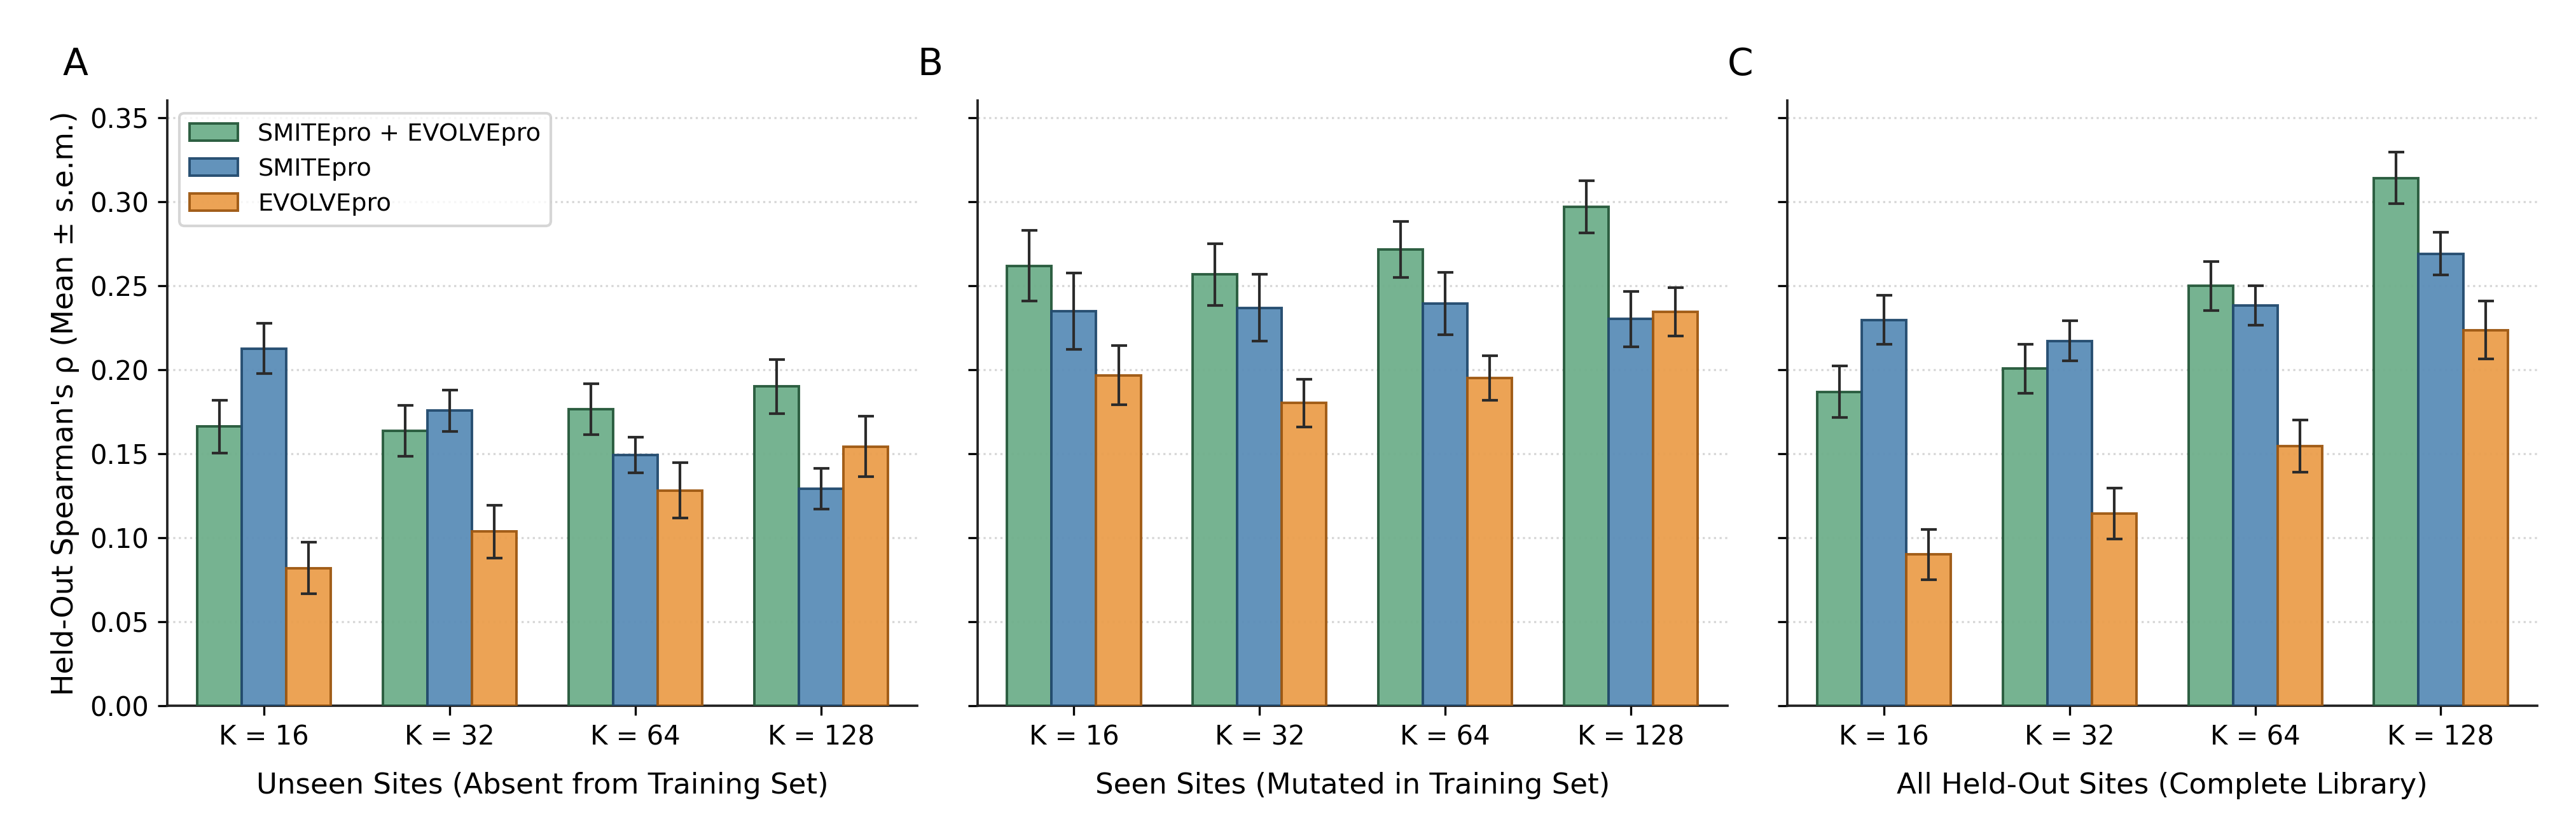
\includegraphics[width=\linewidth]{final_figures/supp_site_scaling_k.png}
    \caption{Site-partitioned held-out Spearman's rank correlation ($\rho \pm \text{s.e.m.}$) scaling across training set sizes $K \in \{16, 32, 64, 128\}$ over the 106 ProteinGym benchmark assays ($\ge 100$ mutated positions). (A) Unseen sites (positions absent from the $K$-variant training set). (B) Seen sites (positions where another substitution was included in the $K$-variant training set). (C) All held-out sites combined across the complete unscreened library.}
    \label{fig:supp-site-scaling}
\end{figure}

\vspace{1em}
\textbf{Prospective HpaBC Ensemble Candidates vs. Prior Training Mutants} \\
To place the prospective 20-variant ensemble screens (Figure~\ref{fig:fig4}) in the context of the experimental training data available on each parental HpaB background~\cite{gutierrez2026monooxygenase}, Figure~\ref{fig:supp-hpab-priors} overlays all single-amino-acid substitutions present in the training set on each of the six backgrounds alongside the 119 prospectively assayed ensemble candidates (with individual stage-by-stage views provided in Supplementary Figures \texttt{supp\_hpab\_stage1\_WT} through \texttt{supp\_hpab\_stage6\_I29V\_A199P\_D354K\_H454Q\_H372P}). On the wild-type background (Round 1), the training set contained 329 previously measured zero-shot single substitutions (including A199P at $5.37\times$ WT, G295T at $5.28\times$ WT, H454Q at $2.79\times$ WT, I29V at $2.43\times$ WT, and H372P at $1.80\times$ WT), all of which were excluded from the unscreened candidate pool. On the evolved backgrounds, the training set contained rational combinations of those initial hits: 5 single-mutant steps on A199P (Round 2, led by I29V at $13.38\times$ WT), 3 on I29V+A199P (Round 3, led by L303H at $18.14\times$ WT), 2 on I29V+A199P+D354K (Round 4, led by G122A at $8.91\times$ WT), 0 on I29V+A199P+D354K+G122A (Round 5), and 6 on I29V+A199P+D354K+H454Q+H372P (Round 6, led by S237C at $42.80\times$ WT and T114S at $41.90\times$ WT). Searching only the remaining unscreened sequence space, the SMITEpro--EVOLVEpro ensemble discovered novel substitutions that exceeded every prior training single mutant in Rounds 3, 4, and 5 and matched the top prior stacked variant in Round 6 (A8R at $42.49\times$ WT).

\begin{figure}[htbp]
    \centering
    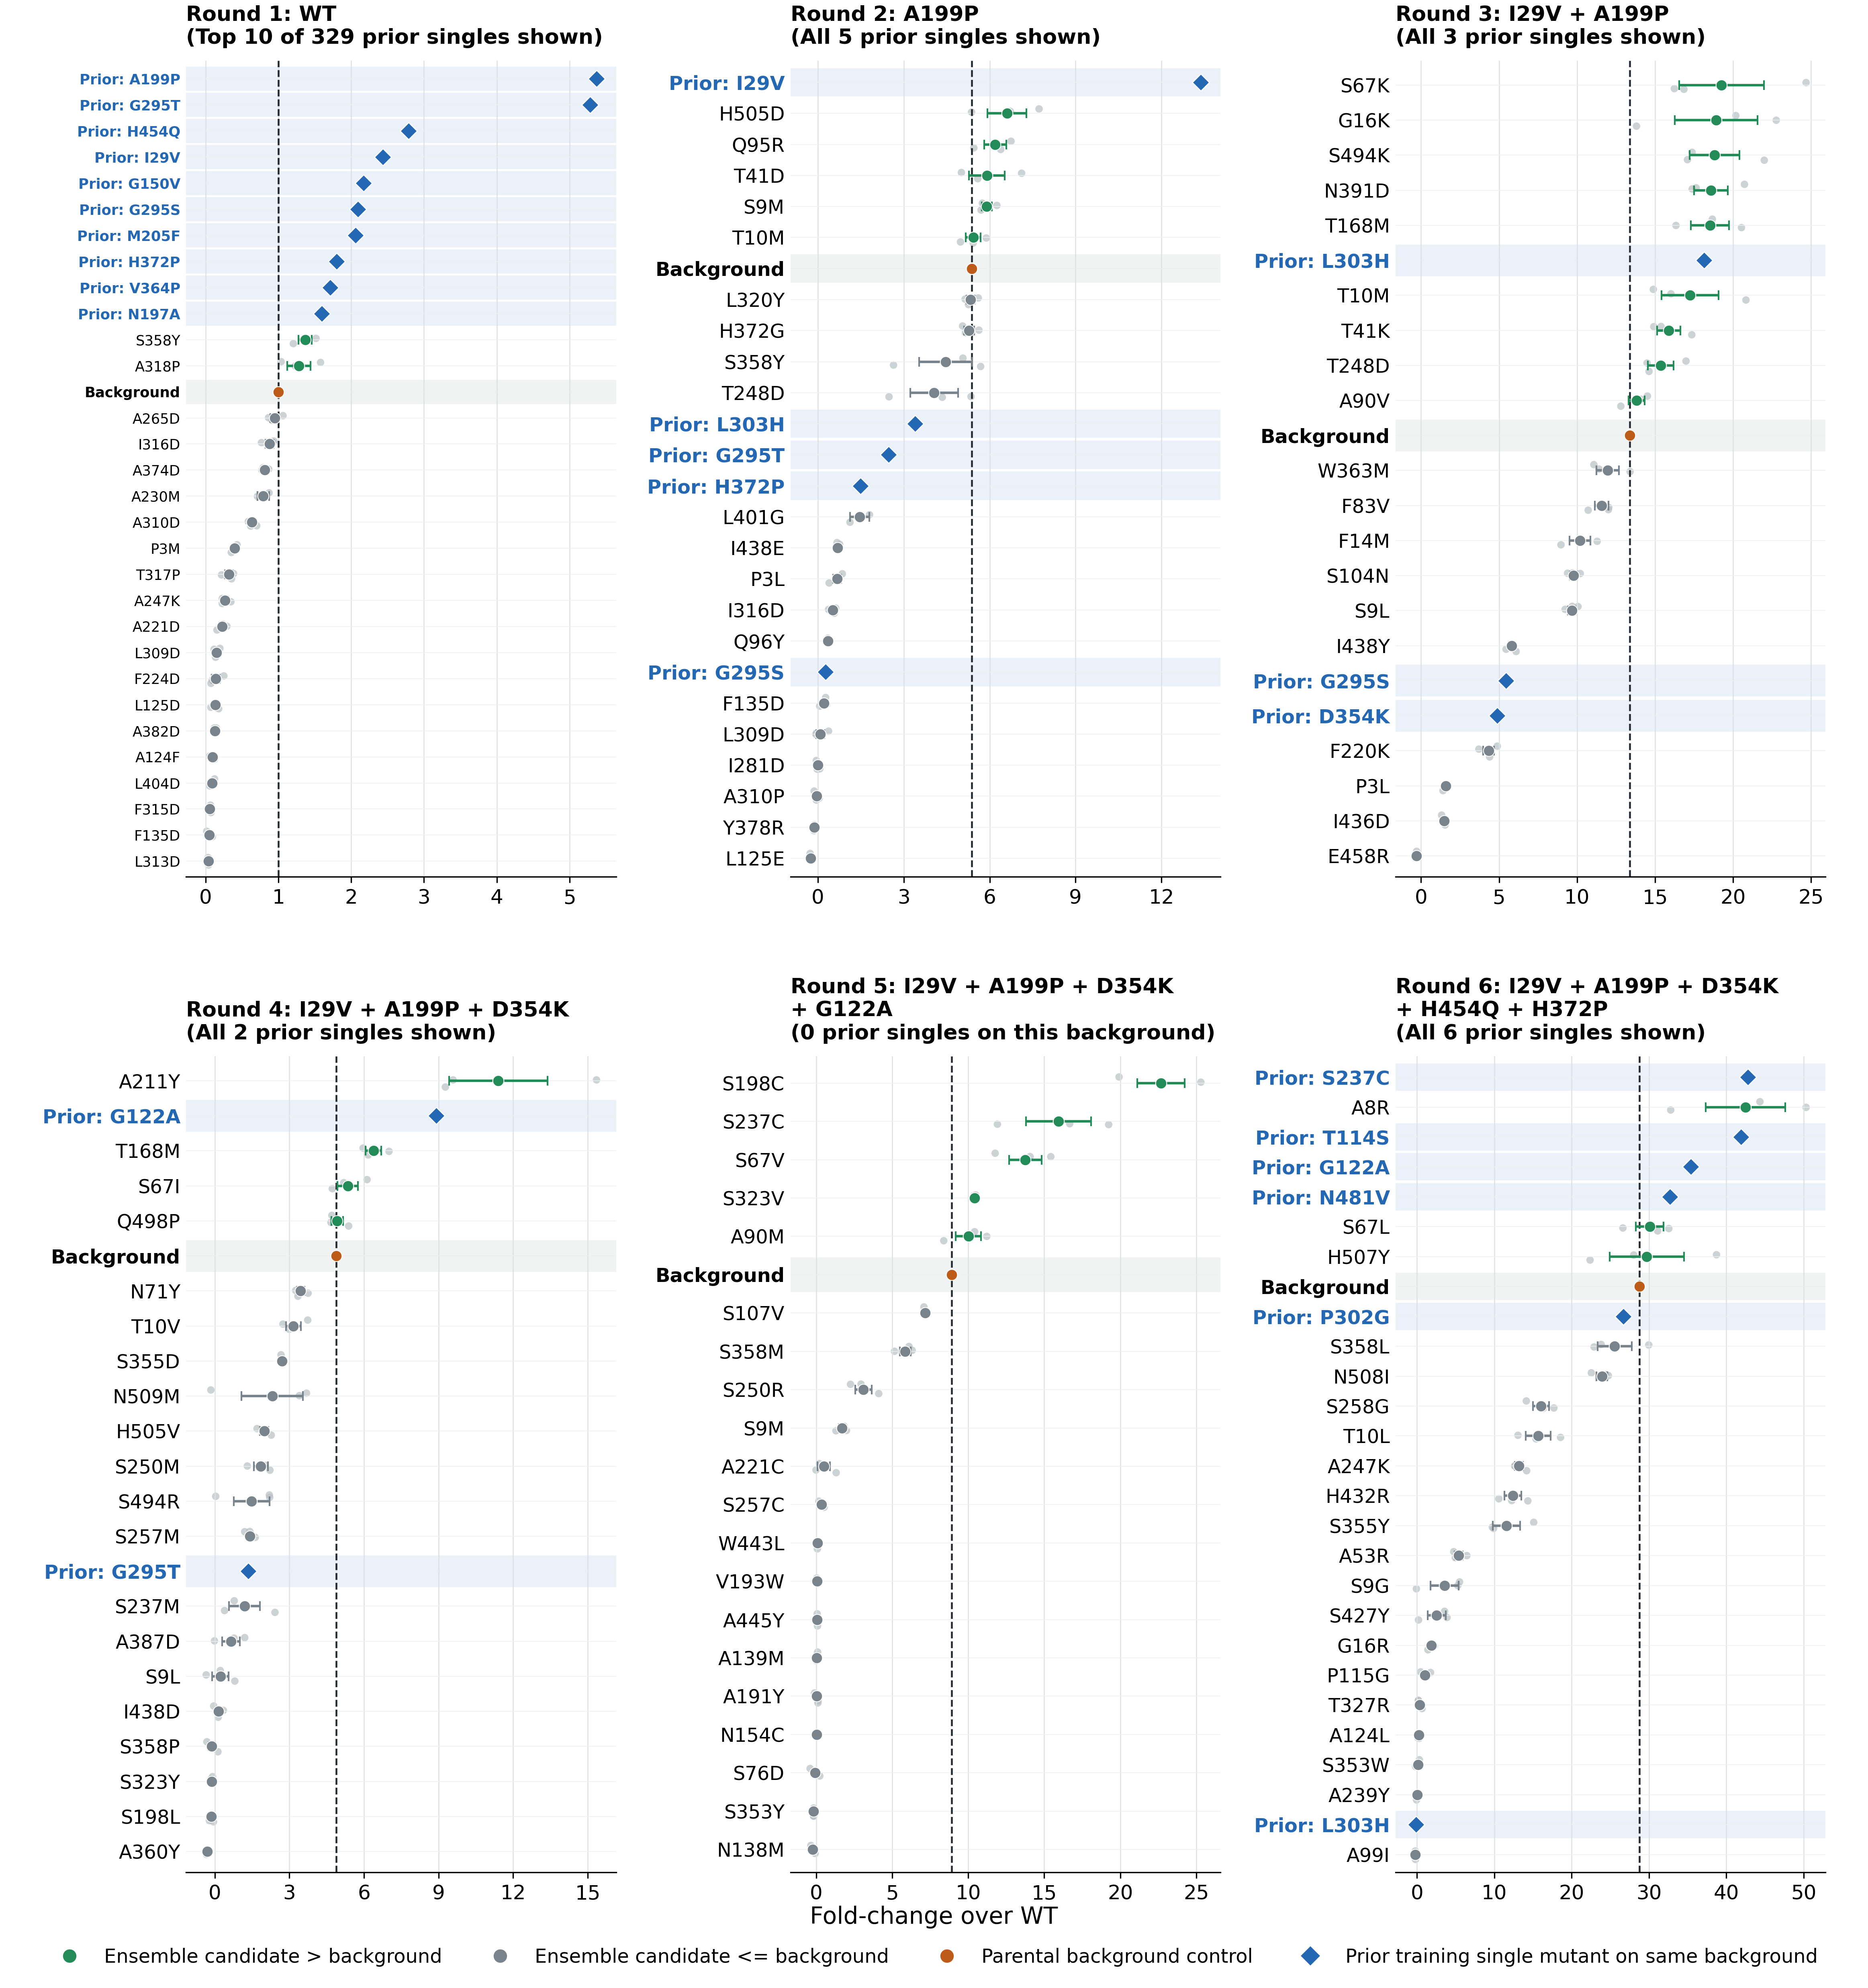
\includegraphics[width=0.99\linewidth]{final_figures/supp_hpab_all_stages_with_priors.png}
    \caption{Comparison of prospectively selected SMITEpro--EVOLVEpro ensemble candidates against prior training single mutants across all six HpaB parental backgrounds. Green and gray circles ($\pm\text{s.e.m.}$, with light gray replicate dots) show the 119 prospectively assayed ensemble candidates above or at/below the matched parental background (orange circle and vertical dashed line). Blue diamonds with shaded rows mark single-amino-acid substitutions on the same parental background that were already present in the training set (top 10 of 329 prior WT single mutants shown in Round 1; all prior single mutants shown in Rounds 2--6).}
    \label{fig:supp-hpab-priors}
\end{figure}

\end{appendices}
\end{document}